% Options for packages loaded elsewhere
\PassOptionsToPackage{unicode}{hyperref}
\PassOptionsToPackage{hyphens}{url}
%
\documentclass[
]{article}
\usepackage{amsmath,amssymb}
\usepackage{iftex}
\ifPDFTeX
  \usepackage[T1]{fontenc}
  \usepackage[utf8]{inputenc}
  \usepackage{textcomp} % provide euro and other symbols
\else % if luatex or xetex
  \usepackage{unicode-math} % this also loads fontspec
  \defaultfontfeatures{Scale=MatchLowercase}
  \defaultfontfeatures[\rmfamily]{Ligatures=TeX,Scale=1}
\fi
\usepackage{lmodern}
\ifPDFTeX\else
  % xetex/luatex font selection
\fi
% Use upquote if available, for straight quotes in verbatim environments
\IfFileExists{upquote.sty}{\usepackage{upquote}}{}
\IfFileExists{microtype.sty}{% use microtype if available
  \usepackage[]{microtype}
  \UseMicrotypeSet[protrusion]{basicmath} % disable protrusion for tt fonts
}{}
\makeatletter
\@ifundefined{KOMAClassName}{% if non-KOMA class
  \IfFileExists{parskip.sty}{%
    \usepackage{parskip}
  }{% else
    \setlength{\parindent}{0pt}
    \setlength{\parskip}{6pt plus 2pt minus 1pt}}
}{% if KOMA class
  \KOMAoptions{parskip=half}}
\makeatother
\usepackage{xcolor}
\usepackage[margin=1in]{geometry}
\usepackage{color}
\usepackage{fancyvrb}
\newcommand{\VerbBar}{|}
\newcommand{\VERB}{\Verb[commandchars=\\\{\}]}
\DefineVerbatimEnvironment{Highlighting}{Verbatim}{commandchars=\\\{\}}
% Add ',fontsize=\small' for more characters per line
\usepackage{framed}
\definecolor{shadecolor}{RGB}{248,248,248}
\newenvironment{Shaded}{\begin{snugshade}}{\end{snugshade}}
\newcommand{\AlertTok}[1]{\textcolor[rgb]{0.94,0.16,0.16}{#1}}
\newcommand{\AnnotationTok}[1]{\textcolor[rgb]{0.56,0.35,0.01}{\textbf{\textit{#1}}}}
\newcommand{\AttributeTok}[1]{\textcolor[rgb]{0.13,0.29,0.53}{#1}}
\newcommand{\BaseNTok}[1]{\textcolor[rgb]{0.00,0.00,0.81}{#1}}
\newcommand{\BuiltInTok}[1]{#1}
\newcommand{\CharTok}[1]{\textcolor[rgb]{0.31,0.60,0.02}{#1}}
\newcommand{\CommentTok}[1]{\textcolor[rgb]{0.56,0.35,0.01}{\textit{#1}}}
\newcommand{\CommentVarTok}[1]{\textcolor[rgb]{0.56,0.35,0.01}{\textbf{\textit{#1}}}}
\newcommand{\ConstantTok}[1]{\textcolor[rgb]{0.56,0.35,0.01}{#1}}
\newcommand{\ControlFlowTok}[1]{\textcolor[rgb]{0.13,0.29,0.53}{\textbf{#1}}}
\newcommand{\DataTypeTok}[1]{\textcolor[rgb]{0.13,0.29,0.53}{#1}}
\newcommand{\DecValTok}[1]{\textcolor[rgb]{0.00,0.00,0.81}{#1}}
\newcommand{\DocumentationTok}[1]{\textcolor[rgb]{0.56,0.35,0.01}{\textbf{\textit{#1}}}}
\newcommand{\ErrorTok}[1]{\textcolor[rgb]{0.64,0.00,0.00}{\textbf{#1}}}
\newcommand{\ExtensionTok}[1]{#1}
\newcommand{\FloatTok}[1]{\textcolor[rgb]{0.00,0.00,0.81}{#1}}
\newcommand{\FunctionTok}[1]{\textcolor[rgb]{0.13,0.29,0.53}{\textbf{#1}}}
\newcommand{\ImportTok}[1]{#1}
\newcommand{\InformationTok}[1]{\textcolor[rgb]{0.56,0.35,0.01}{\textbf{\textit{#1}}}}
\newcommand{\KeywordTok}[1]{\textcolor[rgb]{0.13,0.29,0.53}{\textbf{#1}}}
\newcommand{\NormalTok}[1]{#1}
\newcommand{\OperatorTok}[1]{\textcolor[rgb]{0.81,0.36,0.00}{\textbf{#1}}}
\newcommand{\OtherTok}[1]{\textcolor[rgb]{0.56,0.35,0.01}{#1}}
\newcommand{\PreprocessorTok}[1]{\textcolor[rgb]{0.56,0.35,0.01}{\textit{#1}}}
\newcommand{\RegionMarkerTok}[1]{#1}
\newcommand{\SpecialCharTok}[1]{\textcolor[rgb]{0.81,0.36,0.00}{\textbf{#1}}}
\newcommand{\SpecialStringTok}[1]{\textcolor[rgb]{0.31,0.60,0.02}{#1}}
\newcommand{\StringTok}[1]{\textcolor[rgb]{0.31,0.60,0.02}{#1}}
\newcommand{\VariableTok}[1]{\textcolor[rgb]{0.00,0.00,0.00}{#1}}
\newcommand{\VerbatimStringTok}[1]{\textcolor[rgb]{0.31,0.60,0.02}{#1}}
\newcommand{\WarningTok}[1]{\textcolor[rgb]{0.56,0.35,0.01}{\textbf{\textit{#1}}}}
\usepackage{graphicx}
\makeatletter
\def\maxwidth{\ifdim\Gin@nat@width>\linewidth\linewidth\else\Gin@nat@width\fi}
\def\maxheight{\ifdim\Gin@nat@height>\textheight\textheight\else\Gin@nat@height\fi}
\makeatother
% Scale images if necessary, so that they will not overflow the page
% margins by default, and it is still possible to overwrite the defaults
% using explicit options in \includegraphics[width, height, ...]{}
\setkeys{Gin}{width=\maxwidth,height=\maxheight,keepaspectratio}
% Set default figure placement to htbp
\makeatletter
\def\fps@figure{htbp}
\makeatother
\setlength{\emergencystretch}{3em} % prevent overfull lines
\providecommand{\tightlist}{%
  \setlength{\itemsep}{0pt}\setlength{\parskip}{0pt}}
\setcounter{secnumdepth}{-\maxdimen} % remove section numbering
\ifLuaTeX
  \usepackage{selnolig}  % disable illegal ligatures
\fi
\IfFileExists{bookmark.sty}{\usepackage{bookmark}}{\usepackage{hyperref}}
\IfFileExists{xurl.sty}{\usepackage{xurl}}{} % add URL line breaks if available
\urlstyle{same}
\hypersetup{
  pdftitle={Reclassifying NBA Player Postions Pt. 3 - Clustering Analysis Results},
  pdfauthor={Mike Kaminski},
  hidelinks,
  pdfcreator={LaTeX via pandoc}}

\title{Reclassifying NBA Player Postions Pt. 3 - Clustering Analysis
Results}
\author{Mike Kaminski}
\date{2023-06-23}

\begin{document}
\maketitle

\hypertarget{libraries}{%
\section{Libraries}\label{libraries}}

\begin{Shaded}
\begin{Highlighting}[]
\FunctionTok{library}\NormalTok{(tidymodels) }\CommentTok{\# broom, dials, parsnip, tune, workflows, yardstick}
\FunctionTok{library}\NormalTok{(tidyverse) }\CommentTok{\#ggplot2, dplyr, tidyr, readr, purr, tibble, stringr, lubridate}
\FunctionTok{library}\NormalTok{(gghighlight)}
\end{Highlighting}
\end{Shaded}

\hypertarget{read-in-the-data}{%
\section{Read in the Data}\label{read-in-the-data}}

\begin{Shaded}
\begin{Highlighting}[]
\NormalTok{NBACleanData }\OtherTok{\textless{}{-}} \FunctionTok{read\_csv}\NormalTok{(}\StringTok{"Data/model0623.csv"}\NormalTok{,}\AttributeTok{show\_col\_types =} \ConstantTok{FALSE}\NormalTok{) }\SpecialCharTok{\%\textgreater{}\%} \FunctionTok{select}\NormalTok{(}\SpecialCharTok{{-}}\DecValTok{1}\NormalTok{)}
\NormalTok{model\_df }\OtherTok{\textless{}{-}}\NormalTok{  NBACleanData }\SpecialCharTok{\%\textgreater{}\%} \FunctionTok{select}\NormalTok{(}\SpecialCharTok{{-}}\DecValTok{80}\NormalTok{) }\SpecialCharTok{\%\textgreater{}\%}
  \FunctionTok{mutate}\NormalTok{(}\AttributeTok{Year =} \FunctionTok{as.character}\NormalTok{(Year)) }\SpecialCharTok{\%\textgreater{}\%}
  \FunctionTok{mutate}\NormalTok{(}\FunctionTok{across}\NormalTok{(}\FunctionTok{where}\NormalTok{(is.numeric), }\SpecialCharTok{\textasciitilde{}}\FunctionTok{as.numeric}\NormalTok{(}\FunctionTok{scale}\NormalTok{(.))))}
\end{Highlighting}
\end{Shaded}

From Pt.2 of the project, I decided to use 7 clusters. Using PCA didn't
really provide improved results in the dataset, plus I need to be able
to explain the results in a concise format. Therefore, I've opted to not
use PCA to reduce dimensionality. I've also decided to use kmeans over
hierarchical, as I think it will be a little bit easier to interpret.

\hypertarget{modeling}{%
\section{Modeling}\label{modeling}}

From the last part, here is the model

\begin{Shaded}
\begin{Highlighting}[]
\FunctionTok{set.seed}\NormalTok{(}\DecValTok{1234}\NormalTok{)}

\NormalTok{nba\_clust }\OtherTok{\textless{}{-}} \FunctionTok{kmeans}\NormalTok{(model\_df }\SpecialCharTok{\%\textgreater{}\%} \FunctionTok{select}\NormalTok{(}\SpecialCharTok{{-}}\FunctionTok{c}\NormalTok{(}\DecValTok{1}\SpecialCharTok{:}\DecValTok{4}\NormalTok{)),}
                    \AttributeTok{iter.max =} \DecValTok{500}\NormalTok{ , }
                    \AttributeTok{nstart =} \DecValTok{100}\NormalTok{ ,}
                    \AttributeTok{centers =} \DecValTok{7}\NormalTok{)}
\end{Highlighting}
\end{Shaded}

\begin{Shaded}
\begin{Highlighting}[]
\FunctionTok{head}\NormalTok{(}\FunctionTok{augment}\NormalTok{(nba\_clust, model\_df)[, }\FunctionTok{c}\NormalTok{(}\DecValTok{80}\NormalTok{,}\DecValTok{1}\SpecialCharTok{:}\DecValTok{9}\NormalTok{)],}\DecValTok{5}\NormalTok{) }
\end{Highlighting}
\end{Shaded}

\begin{verbatim}
## # A tibble: 5 x 10
##   .cluster Year  Player    Pos   Tm      FG_pp FGA_pp FG_pct_pp ThrP_pp ThrPA_pp
##   <fct>    <chr> <chr>     <chr> <chr>   <dbl>  <dbl>     <dbl>   <dbl>    <dbl>
## 1 5        2001  AC Green  PF    MIA   -0.951  -0.937   -0.178   -1.18    -1.21 
## 2 3        2001  Aaron Mc~ SG    PHI   -0.0855 -0.259    0.309   -0.299   -0.204
## 3 5        2001  Aaron Wi~ PF    NJN   -0.495  -0.543    0.0404  -1.18    -1.27 
## 4 5        2001  Adam Kee~ PF    GSW   -1.73   -1.59    -0.867   -1.11    -1.21 
## 5 5        2001  Adonal F~ C     GSW   -0.996  -0.850   -0.649   -1.18    -1.27
\end{verbatim}

\begin{Shaded}
\begin{Highlighting}[]
\NormalTok{nba\_aug }\OtherTok{\textless{}{-}} \FunctionTok{augment}\NormalTok{(nba\_clust, model\_df) }\SpecialCharTok{\%\textgreater{}\%} 
  \FunctionTok{rename}\NormalTok{(}\AttributeTok{Cluster =}\NormalTok{ .cluster) }\SpecialCharTok{\%\textgreater{}\%}
  \FunctionTok{select}\NormalTok{(}\SpecialCharTok{{-}}\FunctionTok{c}\NormalTok{(}\DecValTok{1}\SpecialCharTok{:}\DecValTok{4}\NormalTok{)) }\SpecialCharTok{\%\textgreater{}\%}
  \FunctionTok{select}\NormalTok{(Cluster, }\FunctionTok{everything}\NormalTok{()) }
\end{Highlighting}
\end{Shaded}

\hypertarget{create-a-dataframe-for-plotting-results}{%
\section{Create a Dataframe for Plotting
Results}\label{create-a-dataframe-for-plotting-results}}

\begin{Shaded}
\begin{Highlighting}[]
\FunctionTok{options}\NormalTok{(}\AttributeTok{scipen =} \DecValTok{99}\NormalTok{)}
\NormalTok{kmeans\_centers }\OtherTok{\textless{}{-}} \FunctionTok{data.frame}\NormalTok{(}\AttributeTok{Cluster =} \FunctionTok{c}\NormalTok{(}\FunctionTok{paste0}\NormalTok{(}\StringTok{\textquotesingle{}Cluster \textquotesingle{}}\NormalTok{, }\DecValTok{1}\SpecialCharTok{:}\DecValTok{7}\NormalTok{)), nba\_clust}\SpecialCharTok{$}\NormalTok{centers) }\SpecialCharTok{\%\textgreater{}\%} \CommentTok{\#creates a column w/ the cluster name}
  \FunctionTok{pivot\_longer}\NormalTok{(}\SpecialCharTok{!}\NormalTok{Cluster, }\AttributeTok{names\_to =} \StringTok{\textquotesingle{}feature\textquotesingle{}}\NormalTok{, }\AttributeTok{values\_to =} \StringTok{\textquotesingle{}center\textquotesingle{}}\NormalTok{) }\SpecialCharTok{\%\textgreater{}\%} \CommentTok{\#pivots longer for easier graphing}
  \FunctionTok{mutate}\NormalTok{(}\AttributeTok{feature =} \FunctionTok{as.factor}\NormalTok{(feature)) }\SpecialCharTok{\%\textgreater{}\%} \CommentTok{\#makes the feature a factor}
  \FunctionTok{mutate}\NormalTok{(}\AttributeTok{Cluster =} \FunctionTok{as.factor}\NormalTok{(Cluster))}
\FunctionTok{head}\NormalTok{(kmeans\_centers)}
\end{Highlighting}
\end{Shaded}

\begin{verbatim}
## # A tibble: 6 x 3
##   Cluster   feature     center
##   <fct>     <fct>        <dbl>
## 1 Cluster 1 FG_pp        1.14 
## 2 Cluster 1 FGA_pp       0.715
## 3 Cluster 1 FG_pct_pp    0.848
## 4 Cluster 1 ThrP_pp     -0.807
## 5 Cluster 1 ThrPA_pp    -0.839
## 6 Cluster 1 ThrP_pct_pp -0.360
\end{verbatim}

\begin{Shaded}
\begin{Highlighting}[]
\NormalTok{final\_df }\OtherTok{\textless{}{-}}\NormalTok{ model\_df }\SpecialCharTok{\%\textgreater{}\%}
  \FunctionTok{select}\NormalTok{(}\FunctionTok{c}\NormalTok{(}\DecValTok{1}\SpecialCharTok{:}\DecValTok{4}\NormalTok{)) }\SpecialCharTok{\%\textgreater{}\%}
  \FunctionTok{cbind}\NormalTok{(nba\_aug) }\SpecialCharTok{\%\textgreater{}\%}
  \FunctionTok{mutate}\NormalTok{(}\AttributeTok{Cluster =} \FunctionTok{as.character}\NormalTok{(Cluster))}

\NormalTok{df\_2022 }\OtherTok{\textless{}{-}}\NormalTok{ final\_df }\SpecialCharTok{\%\textgreater{}\%}
  \FunctionTok{filter}\NormalTok{(Year }\SpecialCharTok{\%in\%} \StringTok{\textquotesingle{}2022\textquotesingle{}}\NormalTok{)}
\end{Highlighting}
\end{Shaded}

The plots below showcase the makeup of each cluster.

\begin{itemize}
\tightlist
\item
  Plot 1: Each stat category is listed on the x-axis and the cluster
  center is listed on the y-axis. The labels on each point represent the
  rank of that cluster within each stat category.

  \begin{itemize}
  \tightlist
  \item
    A rank of 1 in the per game pre 100 possessions, and advanced stat
    categories (suffixed with pp, pg, adv), indicate that players in
    that cluster performed particularly well in that category - with the
    exception being in the personal foul and turnover stat categories
    (PF and TOV), where a high value is less desirable
  \item
    A rank of 1 in the shooting stat category is more informational
    rather than desirable or undesirable. It represents, among other
    stats, the distances where players are taking shots from. For
    example, it helps identify which players/clusters take 3-point shots
    vs shots close to the basket.
  \item
    Looking at Cluster 1, we see that players in this cluster get a lot
    of rebounds (Reb\_T, Reb\_D, Reb\_O) - they have a high cluster
    center and rank first within that category. We also see that they
    commit a lot of fouls and have a poor defensive rating. A high
    cluster center for fouls is undesirable and a low cluster center for
    defensive rating means that these players aren't good at defense
    (more offensive minded).
  \end{itemize}
\item
  Plot 2: This shows the percentage of stats that fall within each rank
  for the cluster

  \begin{itemize}
  \tightlist
  \item
    If there's a high percentage in ranks 1 and 2, it means that the
    cluster includes players that generally perform well. If there's a
    high percentage in ranks 6 and 7, that means that the cluster
    includes players that generally don't contribute as much as the
    others
  \end{itemize}
\item
  Plot 3: This shows the count of traditional NBA positions in each
  cluster.
\end{itemize}

I've included a new position name for each cluster, a summary of each
position (aka cluster), and listed some of the players from the 2022
season that fall into each position.

\hypertarget{function-for-plotting-all-the-clusters}{%
\subsection{Function for plotting all the
clusters}\label{function-for-plotting-all-the-clusters}}

\begin{Shaded}
\begin{Highlighting}[]
\NormalTok{cluster\_plots }\OtherTok{\textless{}{-}} \ControlFlowTok{function}\NormalTok{(cluster\_value) \{}
  
  \CommentTok{\# Geom\_point for rankings in each category}
\NormalTok{  filtered\_data }\OtherTok{\textless{}{-}}\NormalTok{ kmeans\_centers }\SpecialCharTok{\%\textgreater{}\%}
    \FunctionTok{group\_by}\NormalTok{(feature) }\SpecialCharTok{\%\textgreater{}\%}
    \FunctionTok{mutate}\NormalTok{(}\AttributeTok{rank =} \FunctionTok{ifelse}\NormalTok{(}\FunctionTok{as.character}\NormalTok{(feature) }\SpecialCharTok{\%in\%} \FunctionTok{c}\NormalTok{(}\StringTok{\textquotesingle{}PF\_pg\textquotesingle{}}\NormalTok{, }\StringTok{\textquotesingle{}PF\_pp\textquotesingle{}}\NormalTok{, }\StringTok{\textquotesingle{}TOV\_pg\textquotesingle{}}\NormalTok{, }\StringTok{\textquotesingle{}TOV\_pp\textquotesingle{}}\NormalTok{, }\StringTok{\textquotesingle{}TOV\_pct\_adv\textquotesingle{}}\NormalTok{), }
                         \FunctionTok{rank}\NormalTok{(center), }
                         \FunctionTok{rank}\NormalTok{(}\FunctionTok{desc}\NormalTok{(center)))}
\NormalTok{    )}\SpecialCharTok{\%\textgreater{}\%} \CommentTok{\# adjust rank for high values in less desriable stat categories}
    \FunctionTok{arrange}\NormalTok{(}\FunctionTok{case\_when}\NormalTok{(Cluster }\SpecialCharTok{==}\NormalTok{ cluster\_value }\SpecialCharTok{\textasciitilde{}} \DecValTok{1}\NormalTok{, }\ConstantTok{TRUE} \SpecialCharTok{\textasciitilde{}} \DecValTok{2}\NormalTok{), Cluster, rank, }\FunctionTok{desc}\NormalTok{(center)) }\SpecialCharTok{\%\textgreater{}\%}
    \FunctionTok{mutate}\NormalTok{(}\AttributeTok{Cluster =} \FunctionTok{as.character}\NormalTok{(Cluster)) }\SpecialCharTok{\%\textgreater{}\%}
    \FunctionTok{filter}\NormalTok{(Cluster }\SpecialCharTok{==}\NormalTok{ cluster\_value)}
  
\NormalTok{  plot }\OtherTok{\textless{}{-}}\NormalTok{ kmeans\_centers }\SpecialCharTok{\%\textgreater{}\%}
    \FunctionTok{group\_by}\NormalTok{(feature) }\SpecialCharTok{\%\textgreater{}\%}
    \FunctionTok{mutate}\NormalTok{(}\AttributeTok{rank =} \FunctionTok{ifelse}\NormalTok{(}\FunctionTok{as.character}\NormalTok{(feature) }\SpecialCharTok{\%in\%} \FunctionTok{c}\NormalTok{(}\StringTok{\textquotesingle{}PF\_pg\textquotesingle{}}\NormalTok{, }\StringTok{\textquotesingle{}PF\_pp\textquotesingle{}}\NormalTok{, }\StringTok{\textquotesingle{}TOV\_pg\textquotesingle{}}\NormalTok{, }\StringTok{\textquotesingle{}TOV\_pp\textquotesingle{}}\NormalTok{, }\StringTok{\textquotesingle{}TOV\_pct\_adv\textquotesingle{}}\NormalTok{), }
                         \FunctionTok{rank}\NormalTok{(center), }
                         \FunctionTok{rank}\NormalTok{(}\FunctionTok{desc}\NormalTok{(center)))}
\NormalTok{    )}\SpecialCharTok{\%\textgreater{}\%} \CommentTok{\# adjust rank for high values in less desriable stat categories}
    \FunctionTok{arrange}\NormalTok{(}\FunctionTok{case\_when}\NormalTok{(Cluster }\SpecialCharTok{==}\NormalTok{ cluster\_value }\SpecialCharTok{\textasciitilde{}} \DecValTok{1}\NormalTok{, }\ConstantTok{TRUE} \SpecialCharTok{\textasciitilde{}} \DecValTok{2}\NormalTok{), Cluster, rank, }\FunctionTok{desc}\NormalTok{(center)) }\SpecialCharTok{\%\textgreater{}\%}
    \FunctionTok{ggplot}\NormalTok{(}\FunctionTok{aes}\NormalTok{(}\AttributeTok{x =} \FunctionTok{factor}\NormalTok{(feature, }\AttributeTok{levels =} \FunctionTok{unique}\NormalTok{(feature)), }\AttributeTok{y =}\NormalTok{ center, }\AttributeTok{color =}\NormalTok{ cluster\_value)) }\SpecialCharTok{+}
    \FunctionTok{geom\_point}\NormalTok{(}\AttributeTok{color =} \StringTok{"\#5A2D81"}\NormalTok{) }\SpecialCharTok{+}
    \FunctionTok{geom\_text}\NormalTok{(}\AttributeTok{data =}\NormalTok{ filtered\_data, }\FunctionTok{aes}\NormalTok{(}\AttributeTok{label =}\NormalTok{ rank), }\AttributeTok{color =} \StringTok{"black"}\NormalTok{, }\AttributeTok{vjust =} \SpecialCharTok{{-}}\FloatTok{0.5}\NormalTok{) }\SpecialCharTok{+}  \CommentTok{\# Add point labels for rank}
    \FunctionTok{theme\_minimal}\NormalTok{() }\SpecialCharTok{+}
    \FunctionTok{gghighlight}\NormalTok{(Cluster }\SpecialCharTok{==}\NormalTok{ cluster\_value, }\AttributeTok{use\_direct\_label =} \ConstantTok{FALSE}\NormalTok{) }\SpecialCharTok{+}
    \FunctionTok{theme}\NormalTok{(}\AttributeTok{legend.position =} \StringTok{"none"}\NormalTok{,}
          \AttributeTok{axis.text.x =} \FunctionTok{element\_text}\NormalTok{(}\AttributeTok{angle =} \DecValTok{90}\NormalTok{, }\AttributeTok{size =} \DecValTok{9}\NormalTok{, }\AttributeTok{hjust =} \FloatTok{0.5}\NormalTok{),}
          \AttributeTok{axis.title =} \FunctionTok{element\_text}\NormalTok{(}\AttributeTok{hjust =} \FloatTok{0.5}\NormalTok{),}
          \AttributeTok{plot.title =} \FunctionTok{element\_text}\NormalTok{(}\AttributeTok{hjust =} \FloatTok{0.5}\NormalTok{),}
          \AttributeTok{plot.subtitle =} \FunctionTok{element\_text}\NormalTok{(}\AttributeTok{hjust =} \FloatTok{0.5}\NormalTok{)) }\SpecialCharTok{+}
    \FunctionTok{labs}\NormalTok{(}\AttributeTok{x =} \StringTok{"Statistic"}\NormalTok{, }\AttributeTok{y =} \StringTok{"Cluster Center"}\NormalTok{,}
         \AttributeTok{title =} \StringTok{"Visualizing K{-}Means Cluster Makeups"}\NormalTok{,}
         \AttributeTok{subtitle =}\NormalTok{ cluster\_value)}
  
  \FunctionTok{print}\NormalTok{(plot)}
  
  
  \CommentTok{\# Bar Plot for Percentage of Stat Categories in Each Rank}
\NormalTok{  filtered\_data }\OtherTok{\textless{}{-}}\NormalTok{ kmeans\_centers }\SpecialCharTok{\%\textgreater{}\%}
    \FunctionTok{group\_by}\NormalTok{(feature) }\SpecialCharTok{\%\textgreater{}\%}
    \FunctionTok{mutate}\NormalTok{(}\AttributeTok{rank =} \FunctionTok{ifelse}\NormalTok{(}\FunctionTok{as.character}\NormalTok{(feature) }\SpecialCharTok{\%in\%} \FunctionTok{c}\NormalTok{(}\StringTok{\textquotesingle{}PF\_pg\textquotesingle{}}\NormalTok{, }\StringTok{\textquotesingle{}PF\_pp\textquotesingle{}}\NormalTok{, }\StringTok{\textquotesingle{}TOV\_pg\textquotesingle{}}\NormalTok{, }\StringTok{\textquotesingle{}TOV\_pp\textquotesingle{}}\NormalTok{, }\StringTok{\textquotesingle{}TOV\_pct\_adv\textquotesingle{}}\NormalTok{), }
                         \FunctionTok{rank}\NormalTok{(center), }
                         \FunctionTok{rank}\NormalTok{(}\FunctionTok{desc}\NormalTok{(center)))}
\NormalTok{    ) }\SpecialCharTok{\%\textgreater{}\%}
    \FunctionTok{arrange}\NormalTok{(}\FunctionTok{case\_when}\NormalTok{(Cluster }\SpecialCharTok{==}\NormalTok{ cluster\_value }\SpecialCharTok{\textasciitilde{}} \DecValTok{1}\NormalTok{, }\ConstantTok{TRUE} \SpecialCharTok{\textasciitilde{}} \DecValTok{2}\NormalTok{), Cluster, rank, }\FunctionTok{desc}\NormalTok{(center)) }\SpecialCharTok{\%\textgreater{}\%}
    \FunctionTok{mutate}\NormalTok{(}\AttributeTok{Cluster =} \FunctionTok{as.character}\NormalTok{(Cluster)) }\SpecialCharTok{\%\textgreater{}\%}
    \FunctionTok{filter}\NormalTok{(Cluster }\SpecialCharTok{==}\NormalTok{ cluster\_value)}
  
\NormalTok{  plot }\OtherTok{\textless{}{-}}\NormalTok{ kmeans\_centers }\SpecialCharTok{\%\textgreater{}\%}
    \FunctionTok{group\_by}\NormalTok{(feature) }\SpecialCharTok{\%\textgreater{}\%}
    \FunctionTok{mutate}\NormalTok{(}\AttributeTok{rank =} \FunctionTok{ifelse}\NormalTok{(}\FunctionTok{as.character}\NormalTok{(feature) }\SpecialCharTok{\%in\%} \FunctionTok{c}\NormalTok{(}\StringTok{\textquotesingle{}PF\_pg\textquotesingle{}}\NormalTok{, }\StringTok{\textquotesingle{}PF\_pp\textquotesingle{}}\NormalTok{, }\StringTok{\textquotesingle{}TOV\_pg\textquotesingle{}}\NormalTok{, }\StringTok{\textquotesingle{}TOV\_pp\textquotesingle{}}\NormalTok{, }\StringTok{\textquotesingle{}TOV\_pct\_adv\textquotesingle{}}\NormalTok{), }
                         \FunctionTok{rank}\NormalTok{(center), }
                         \FunctionTok{rank}\NormalTok{(}\FunctionTok{desc}\NormalTok{(center)))}
\NormalTok{    ) }\SpecialCharTok{\%\textgreater{}\%}
    \FunctionTok{ungroup}\NormalTok{() }\SpecialCharTok{\%\textgreater{}\%}
    \FunctionTok{select}\NormalTok{(Cluster, rank) }\SpecialCharTok{\%\textgreater{}\%}
    \FunctionTok{group\_by}\NormalTok{(Cluster, rank) }\SpecialCharTok{\%\textgreater{}\%}
    \FunctionTok{summarise}\NormalTok{(}\AttributeTok{count =} \FunctionTok{n}\NormalTok{()) }\SpecialCharTok{\%\textgreater{}\%}
    \FunctionTok{ungroup}\NormalTok{() }\SpecialCharTok{\%\textgreater{}\%}
    \FunctionTok{group\_by}\NormalTok{(Cluster) }\SpecialCharTok{\%\textgreater{}\%}
    \FunctionTok{mutate}\NormalTok{(}\AttributeTok{percentage =}\NormalTok{ count }\SpecialCharTok{/} \FunctionTok{sum}\NormalTok{(count) }\SpecialCharTok{*} \DecValTok{100}\NormalTok{) }\SpecialCharTok{\%\textgreater{}\%}
    \FunctionTok{filter}\NormalTok{(Cluster }\SpecialCharTok{==}\NormalTok{ cluster\_value) }\SpecialCharTok{\%\textgreater{}\%}
    \FunctionTok{ggplot}\NormalTok{(}\FunctionTok{aes}\NormalTok{(}\AttributeTok{x =} \FunctionTok{as.factor}\NormalTok{(rank), }\AttributeTok{y =}\NormalTok{ percentage, }\AttributeTok{fill =} \FunctionTok{as.factor}\NormalTok{(rank))) }\SpecialCharTok{+}
    \FunctionTok{geom\_bar}\NormalTok{(}\AttributeTok{stat =} \StringTok{"identity"}\NormalTok{) }\SpecialCharTok{+}
    \FunctionTok{geom\_text}\NormalTok{(}\FunctionTok{aes}\NormalTok{(}\AttributeTok{label =} \FunctionTok{paste0}\NormalTok{(}\FunctionTok{round}\NormalTok{(percentage, }\DecValTok{0}\NormalTok{), }\StringTok{"\%"}\NormalTok{)), }\AttributeTok{vjust =} \SpecialCharTok{{-}}\FloatTok{0.5}\NormalTok{, }\AttributeTok{color =} \StringTok{"black"}\NormalTok{) }\SpecialCharTok{+}
    \FunctionTok{labs}\NormalTok{(}\AttributeTok{x =} \StringTok{"Rank"}\NormalTok{, }\AttributeTok{y =} \StringTok{"Percentage"}\NormalTok{,}
         \AttributeTok{title =} \StringTok{"Percentage of Stat Categories in Each Rank"}\NormalTok{, }\AttributeTok{subtitle =}\NormalTok{ cluster\_value) }\SpecialCharTok{+}
    \FunctionTok{scale\_fill\_discrete}\NormalTok{(}\AttributeTok{name =} \StringTok{"Rank"}\NormalTok{) }\SpecialCharTok{+}
    \FunctionTok{scale\_x\_discrete}\NormalTok{(}\AttributeTok{limits =} \FunctionTok{as.character}\NormalTok{(}\DecValTok{1}\SpecialCharTok{:}\DecValTok{7}\NormalTok{)) }\SpecialCharTok{+}
    \FunctionTok{theme\_minimal}\NormalTok{()}
  
  \FunctionTok{print}\NormalTok{(plot)}
  
  \CommentTok{\#Bar plot that shows count of traditional positions in each cluster}
\NormalTok{  df\_2022 }\OtherTok{\textless{}{-}}\NormalTok{ final\_df }\SpecialCharTok{\%\textgreater{}\%}
    \FunctionTok{filter}\NormalTok{(Year }\SpecialCharTok{\%in\%} \StringTok{\textquotesingle{}2022\textquotesingle{}}\NormalTok{)}
  
\NormalTok{  count\_df }\OtherTok{\textless{}{-}}\NormalTok{ df\_2022 }\SpecialCharTok{\%\textgreater{}\%}
    \FunctionTok{filter}\NormalTok{(Cluster }\SpecialCharTok{==} \FunctionTok{substr}\NormalTok{(cluster\_value, }\FunctionTok{nchar}\NormalTok{(cluster\_value), }\FunctionTok{nchar}\NormalTok{(cluster\_value))) }\SpecialCharTok{\%\textgreater{}\%}
    \FunctionTok{group\_by}\NormalTok{(Pos) }\SpecialCharTok{\%\textgreater{}\%}
    \FunctionTok{summarise}\NormalTok{(}\AttributeTok{count =} \FunctionTok{n}\NormalTok{()) }\SpecialCharTok{\%\textgreater{}\%}
    \FunctionTok{ungroup}\NormalTok{() }\SpecialCharTok{\%\textgreater{}\%}
    \FunctionTok{arrange}\NormalTok{(}\FunctionTok{desc}\NormalTok{(count))}
  
\NormalTok{  plot }\OtherTok{\textless{}{-}} \FunctionTok{ggplot}\NormalTok{(count\_df, }\FunctionTok{aes}\NormalTok{(}\AttributeTok{x =} \FunctionTok{reorder}\NormalTok{(Pos, }\SpecialCharTok{{-}}\NormalTok{count), }\AttributeTok{y =}\NormalTok{ count, }\AttributeTok{fill =}\NormalTok{ Pos)) }\SpecialCharTok{+}
    \FunctionTok{geom\_bar}\NormalTok{(}\AttributeTok{stat =} \StringTok{"identity"}\NormalTok{) }\SpecialCharTok{+}
    \FunctionTok{geom\_text}\NormalTok{(}\FunctionTok{aes}\NormalTok{(}\AttributeTok{label =}\NormalTok{ count), }\AttributeTok{vjust =} \SpecialCharTok{{-}}\FloatTok{0.5}\NormalTok{, }\AttributeTok{color =} \StringTok{"black"}\NormalTok{) }\SpecialCharTok{+}
    \FunctionTok{scale\_fill\_manual}\NormalTok{(}\AttributeTok{values =} \FunctionTok{c}\NormalTok{(}\StringTok{"red"}\NormalTok{, }\StringTok{"blue"}\NormalTok{, }\StringTok{"green"}\NormalTok{, }\StringTok{"yellow"}\NormalTok{, }\StringTok{"orange"}\NormalTok{)) }\SpecialCharTok{+}
    \FunctionTok{labs}\NormalTok{(}\AttributeTok{x =} \StringTok{"Pos"}\NormalTok{, }\AttributeTok{y =} \StringTok{"Count"}\NormalTok{, }\AttributeTok{title =} \FunctionTok{paste0}\NormalTok{(}\StringTok{"Bar Plot of Traditional Positions in "}\NormalTok{, cluster\_value))}
  
  \FunctionTok{print}\NormalTok{(plot)}
\NormalTok{\}}
\end{Highlighting}
\end{Shaded}

\hypertarget{cluster-1}{%
\subsection{Cluster 1}\label{cluster-1}}

MVP Bigs * In 2022, there were 20 players in this cluster,
\textasciitilde5\% - the smallest cluster + Notable players include:
Anthony Davis, Deandre Ayton, Kristaps Porzingis, Rudy Gobert, Domantas
Sabonis, Bam Adebayo + These players are predominately centers with some
power forwards sprinkled in * They rank first or second in
\textasciitilde60\% of the stats, ranking second in \textasciitilde45\%
of the stats and rank second to last or last in \textasciitilde5\% *
They're first or second in almost all rebounding and blocking stats.
They're second in many of the advanced stats including PER, Win Share,
and VORP. They play the second most points and score the second most
points. They take a lot of two point shoots and shoot a lot of free
throws * They only have lower ranks in a few stats. They turn the ball
over a lot and they foul a lot. They have the shortest field goal
distance, which isn't a bad thing, it just means they shoot close to the
basket.

\begin{Shaded}
\begin{Highlighting}[]
\FunctionTok{cluster\_plots}\NormalTok{(}\StringTok{\textquotesingle{}Cluster 1\textquotesingle{}}\NormalTok{)}
\end{Highlighting}
\end{Shaded}

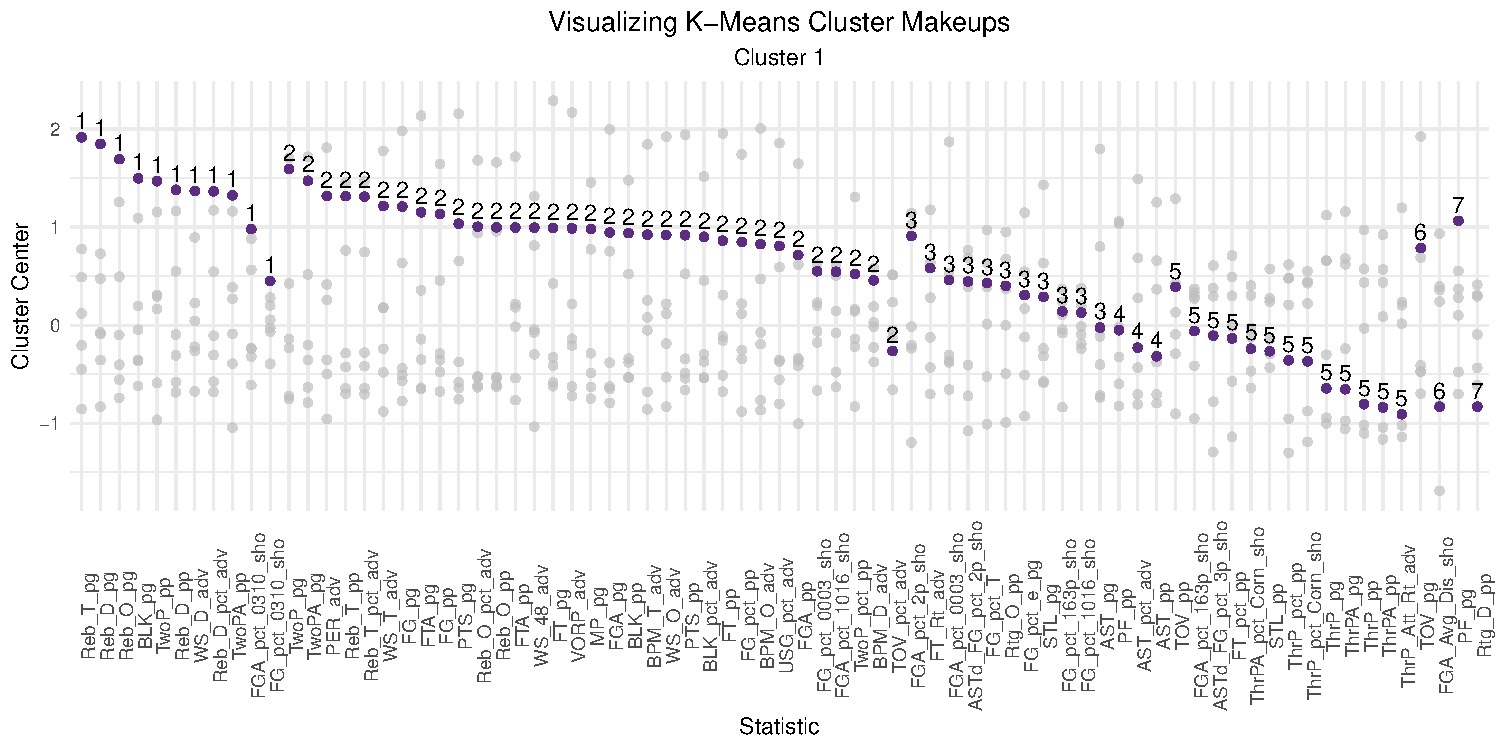
\includegraphics{Reclassifying-NBA-Player-Postions-Pt.-3---Clustering-Analysis-Results_files/figure-latex/unnamed-chunk-2-1.pdf}
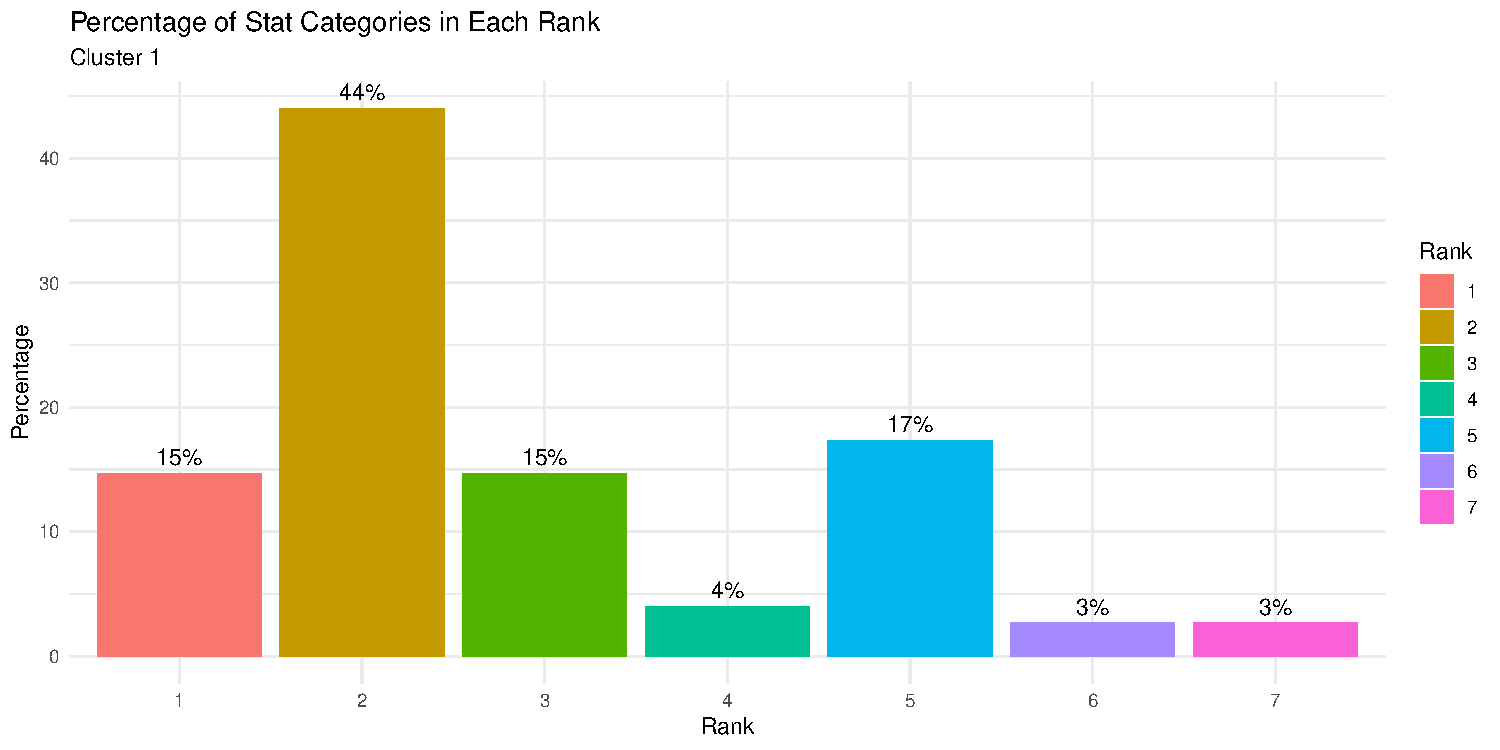
\includegraphics{Reclassifying-NBA-Player-Postions-Pt.-3---Clustering-Analysis-Results_files/figure-latex/unnamed-chunk-2-2.pdf}
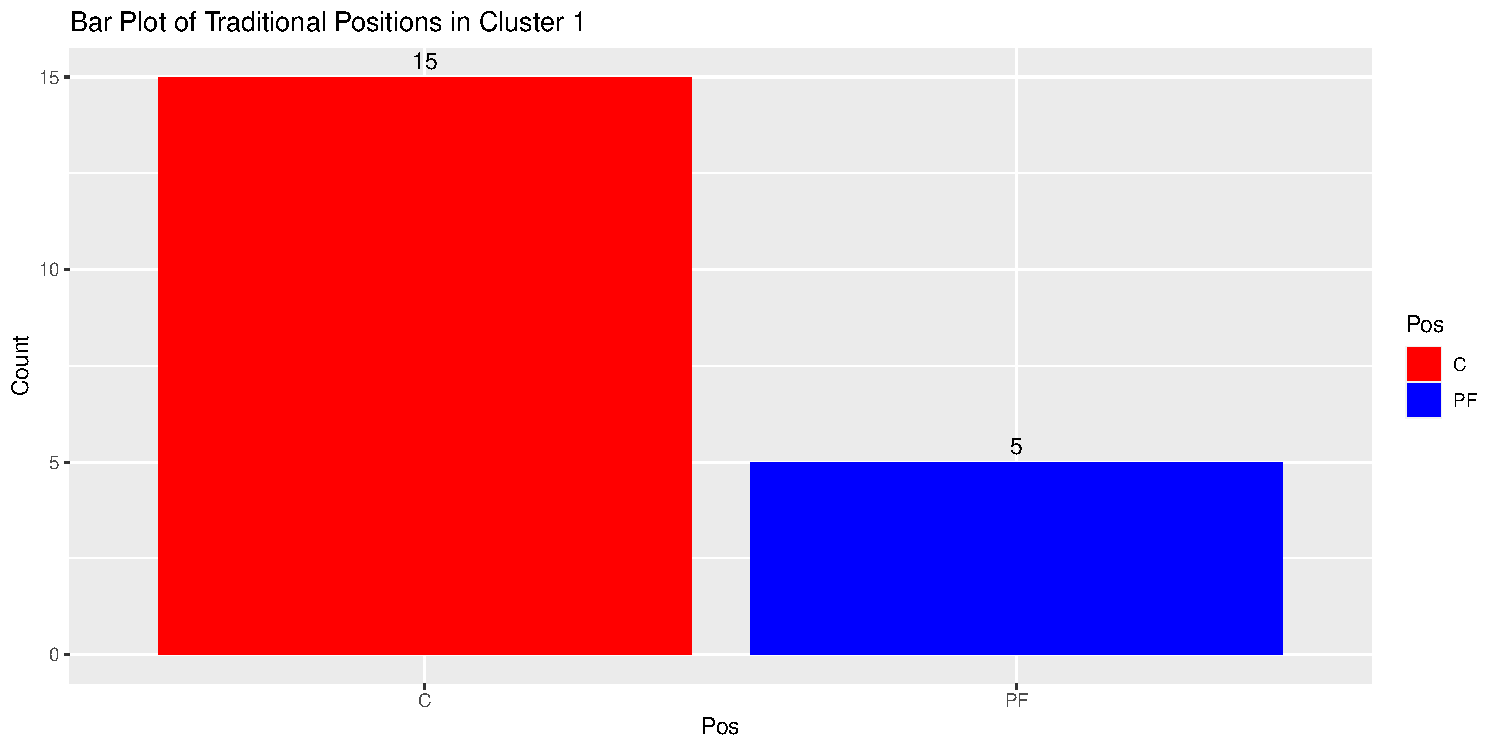
\includegraphics{Reclassifying-NBA-Player-Postions-Pt.-3---Clustering-Analysis-Results_files/figure-latex/unnamed-chunk-2-3.pdf}

\hypertarget{cluster-2}{%
\subsection{Cluster 2}\label{cluster-2}}

\begin{Shaded}
\begin{Highlighting}[]
\FunctionTok{cluster\_plots}\NormalTok{(}\StringTok{\textquotesingle{}Cluster 2\textquotesingle{}}\NormalTok{)}
\end{Highlighting}
\end{Shaded}

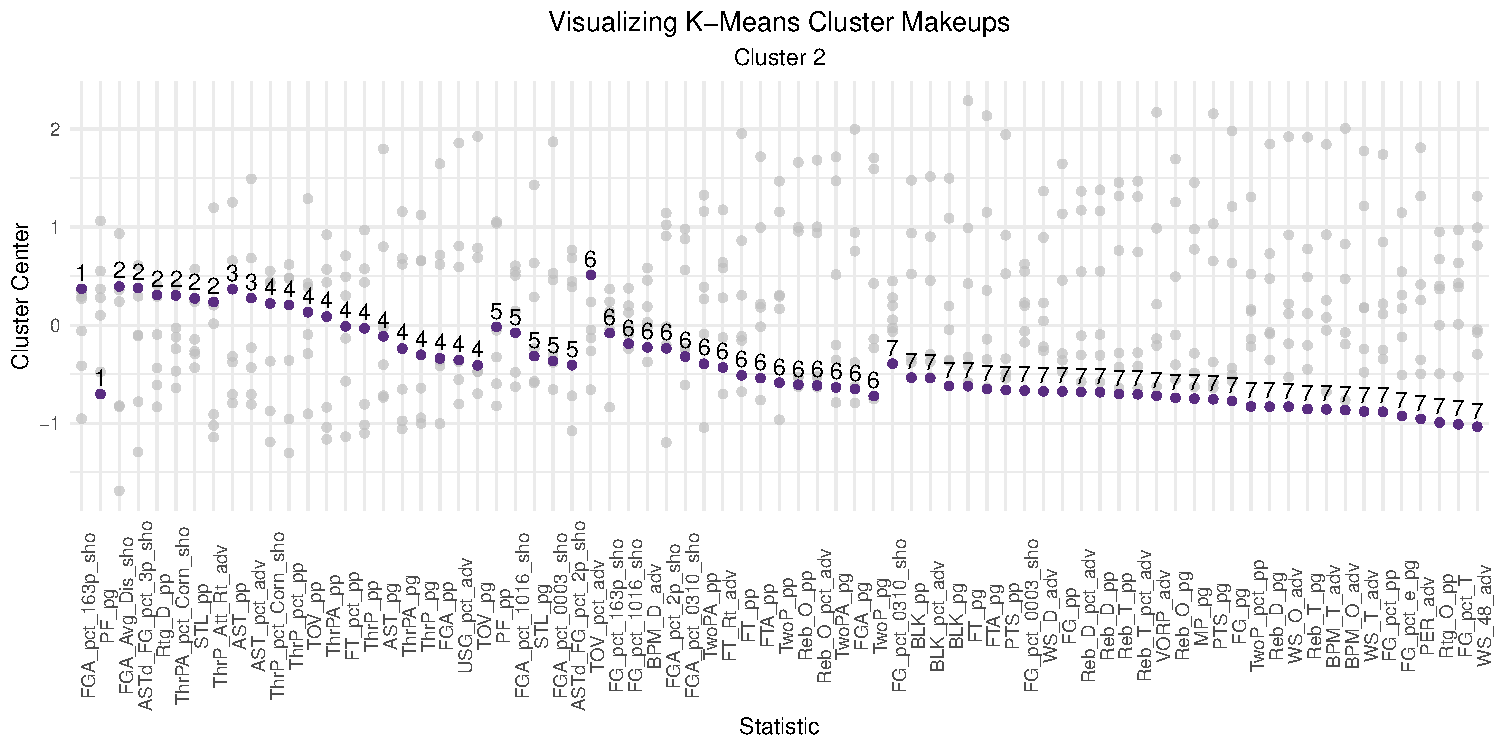
\includegraphics{Reclassifying-NBA-Player-Postions-Pt.-3---Clustering-Analysis-Results_files/figure-latex/unnamed-chunk-3-1.pdf}
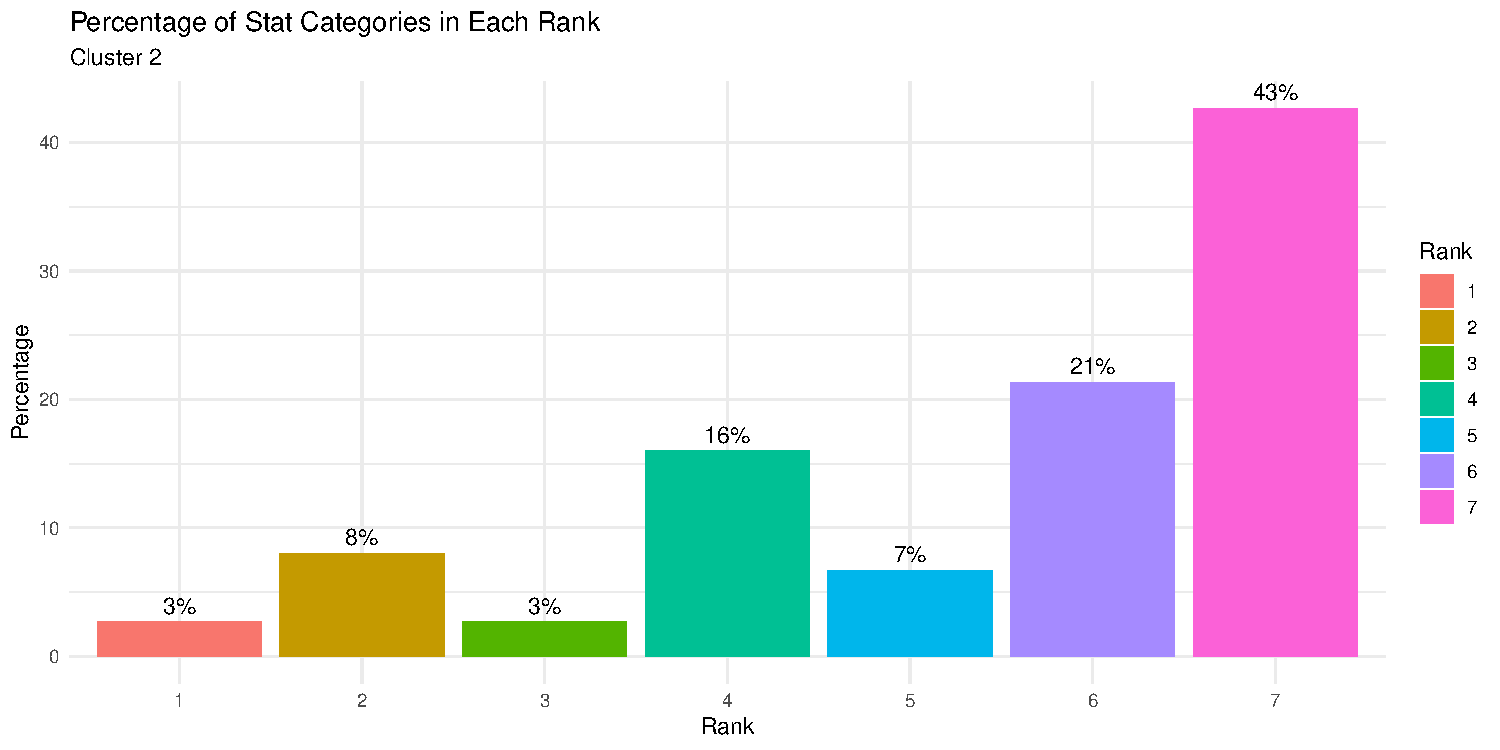
\includegraphics{Reclassifying-NBA-Player-Postions-Pt.-3---Clustering-Analysis-Results_files/figure-latex/unnamed-chunk-3-2.pdf}
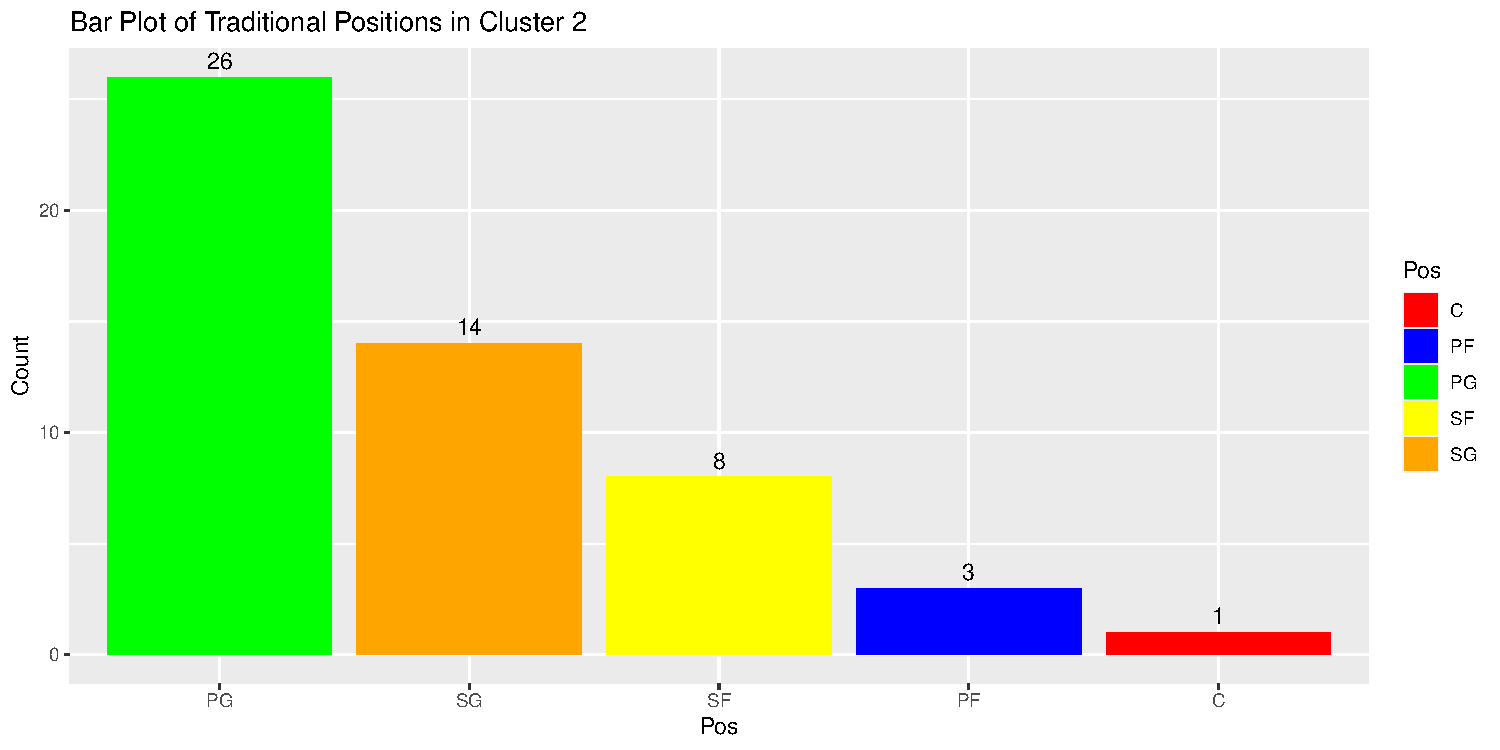
\includegraphics{Reclassifying-NBA-Player-Postions-Pt.-3---Clustering-Analysis-Results_files/figure-latex/unnamed-chunk-3-3.pdf}

\hypertarget{cluster-3}{%
\subsection{Cluster 3}\label{cluster-3}}

\begin{Shaded}
\begin{Highlighting}[]
\FunctionTok{cluster\_plots}\NormalTok{(}\StringTok{\textquotesingle{}Cluster 3\textquotesingle{}}\NormalTok{)}
\end{Highlighting}
\end{Shaded}

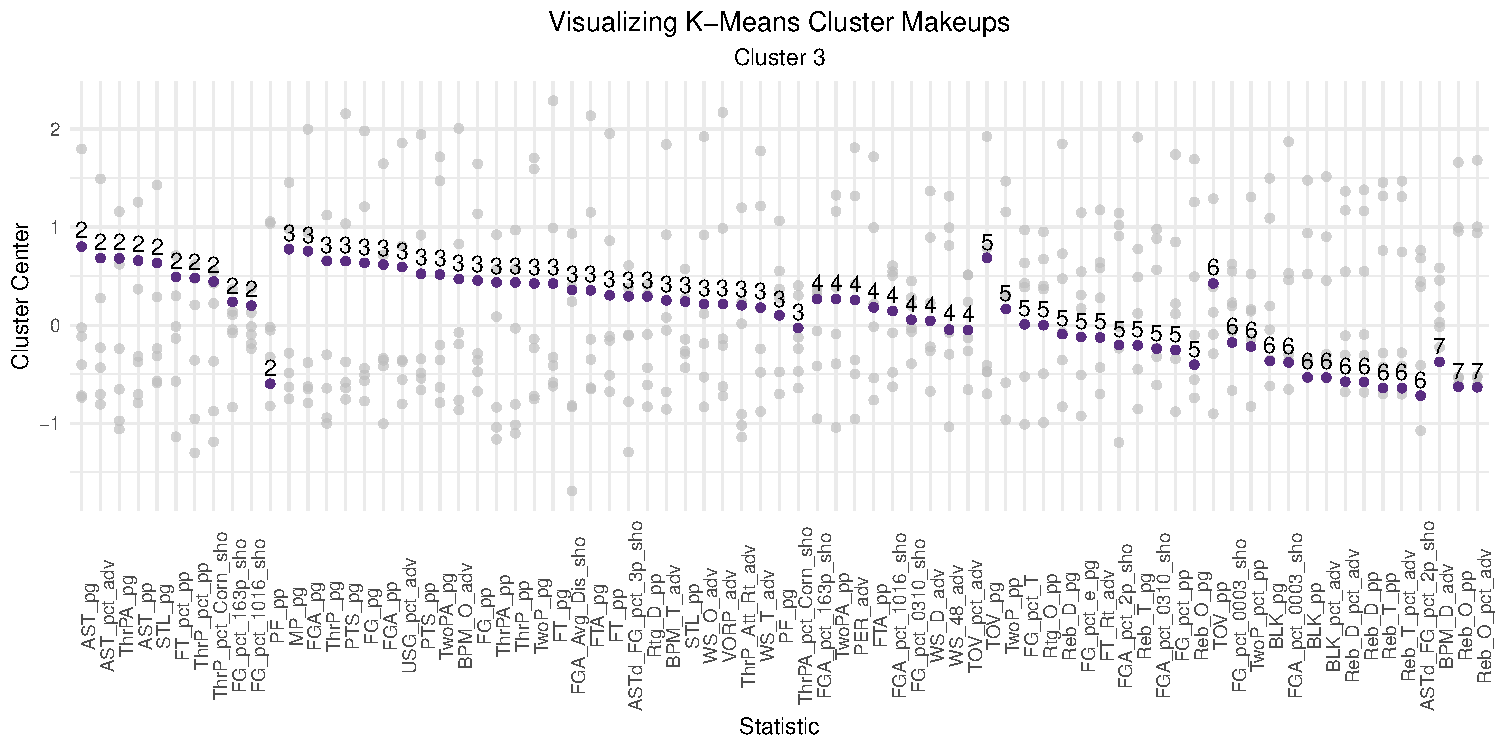
\includegraphics{Reclassifying-NBA-Player-Postions-Pt.-3---Clustering-Analysis-Results_files/figure-latex/unnamed-chunk-4-1.pdf}
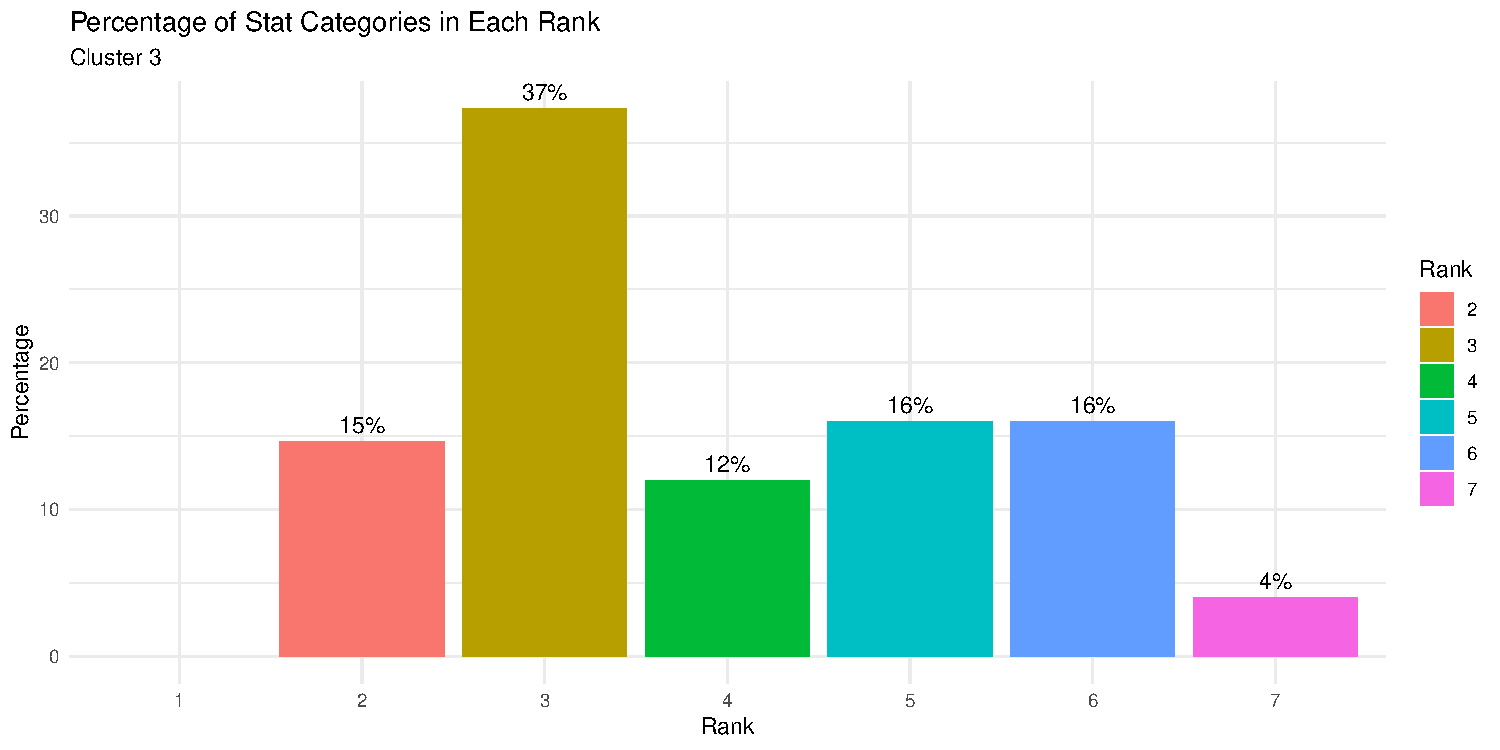
\includegraphics{Reclassifying-NBA-Player-Postions-Pt.-3---Clustering-Analysis-Results_files/figure-latex/unnamed-chunk-4-2.pdf}
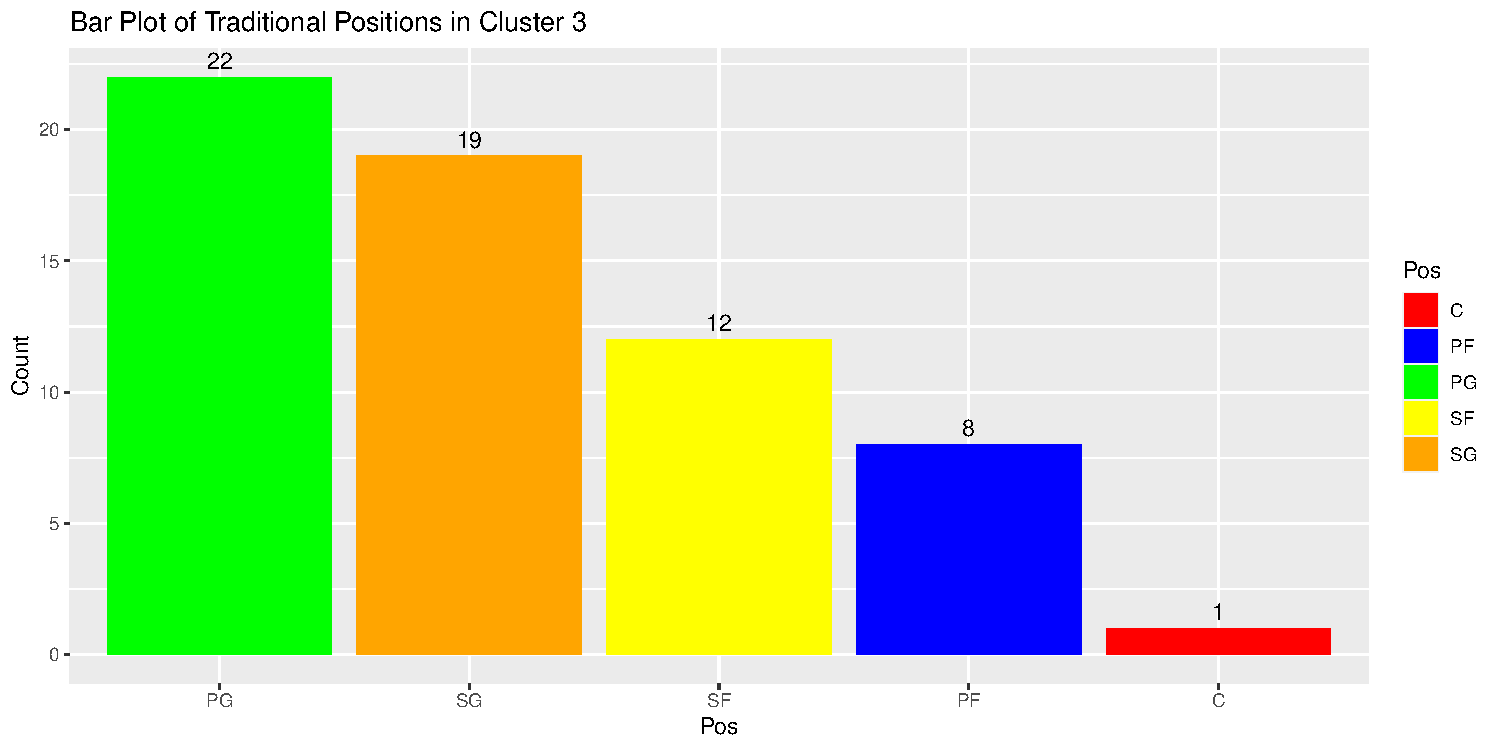
\includegraphics{Reclassifying-NBA-Player-Postions-Pt.-3---Clustering-Analysis-Results_files/figure-latex/unnamed-chunk-4-3.pdf}

\hypertarget{cluster-4}{%
\subsection{Cluster 4}\label{cluster-4}}

\begin{Shaded}
\begin{Highlighting}[]
\FunctionTok{cluster\_plots}\NormalTok{(}\StringTok{\textquotesingle{}Cluster 4\textquotesingle{}}\NormalTok{)}
\end{Highlighting}
\end{Shaded}

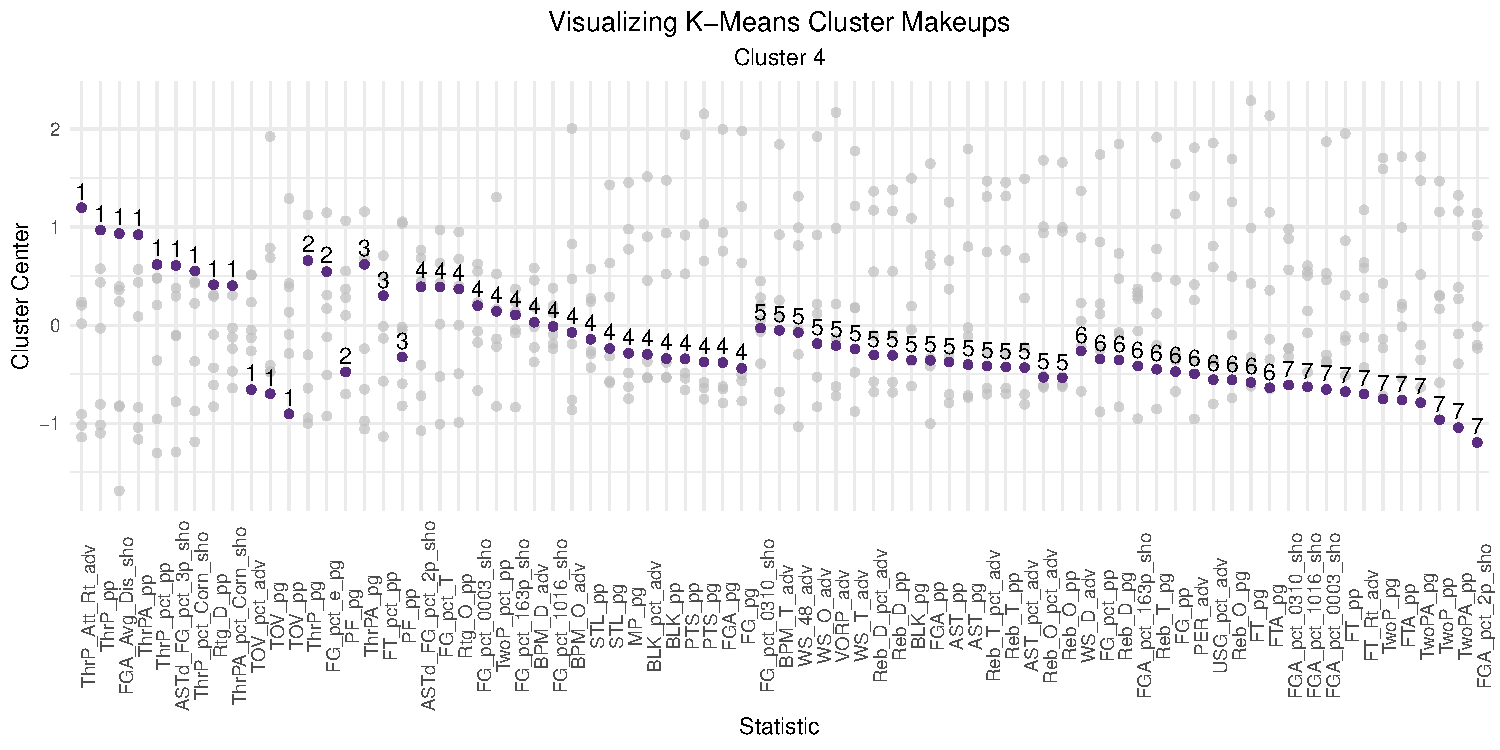
\includegraphics{Reclassifying-NBA-Player-Postions-Pt.-3---Clustering-Analysis-Results_files/figure-latex/unnamed-chunk-5-1.pdf}
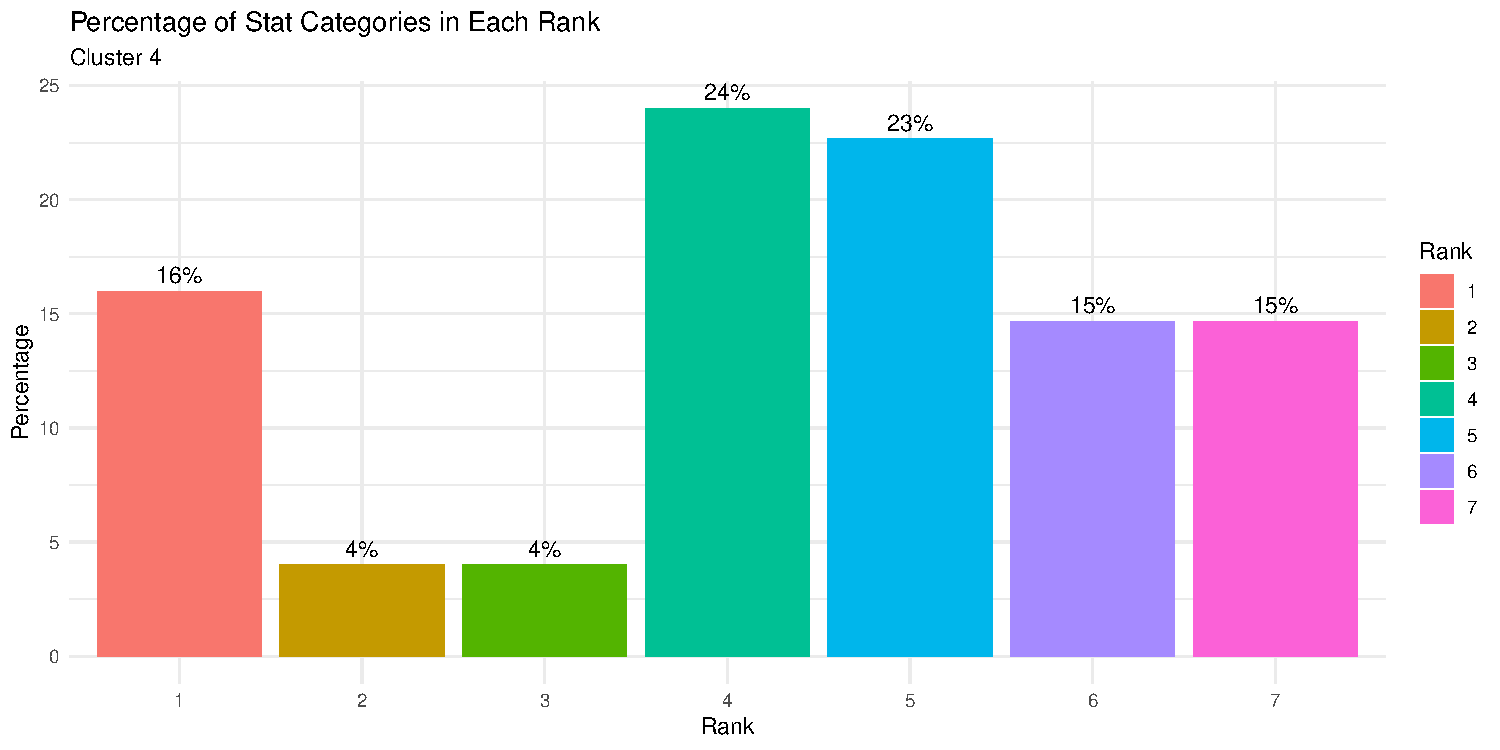
\includegraphics{Reclassifying-NBA-Player-Postions-Pt.-3---Clustering-Analysis-Results_files/figure-latex/unnamed-chunk-5-2.pdf}
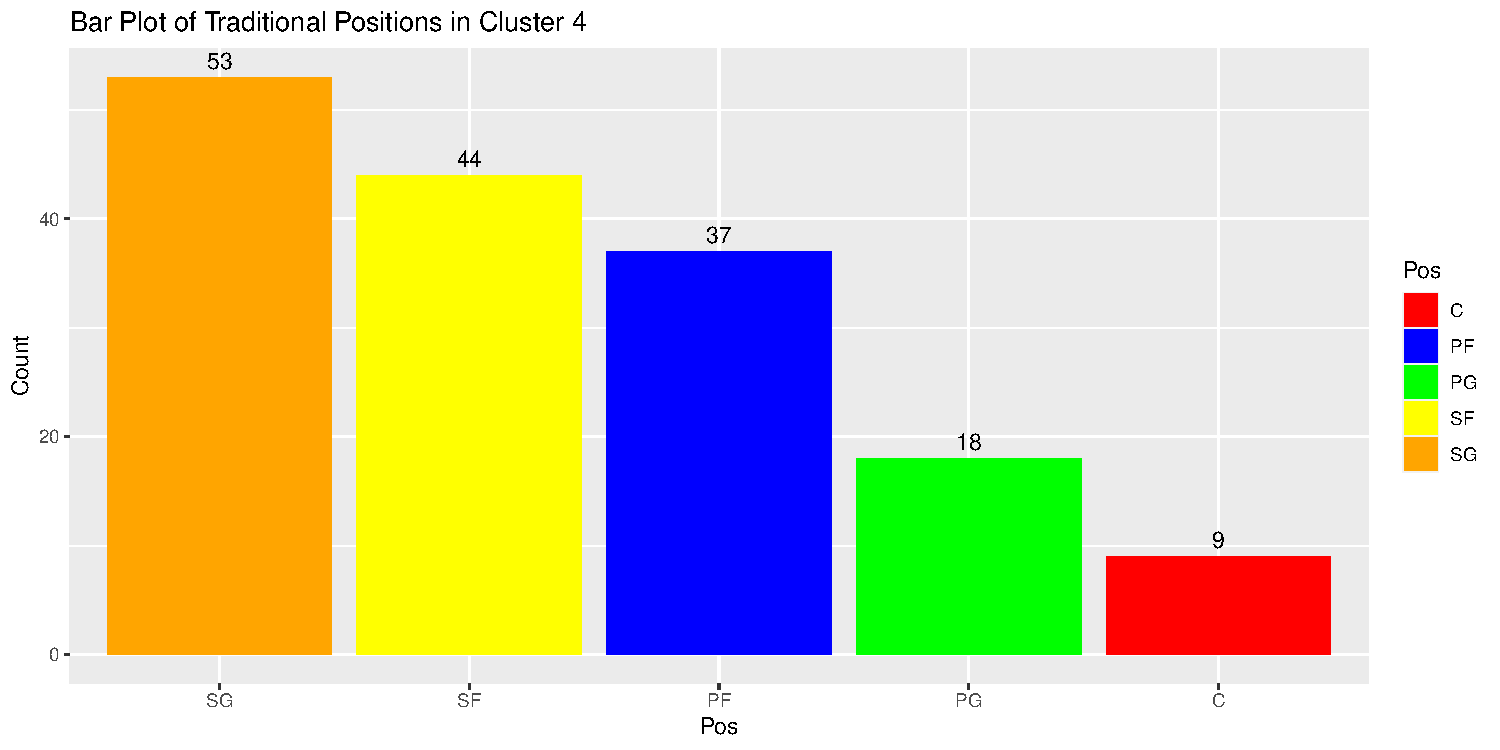
\includegraphics{Reclassifying-NBA-Player-Postions-Pt.-3---Clustering-Analysis-Results_files/figure-latex/unnamed-chunk-5-3.pdf}

\hypertarget{cluster-5}{%
\subsection{Cluster 5}\label{cluster-5}}

\begin{Shaded}
\begin{Highlighting}[]
\FunctionTok{cluster\_plots}\NormalTok{(}\StringTok{\textquotesingle{}Cluster 5\textquotesingle{}}\NormalTok{)}
\end{Highlighting}
\end{Shaded}

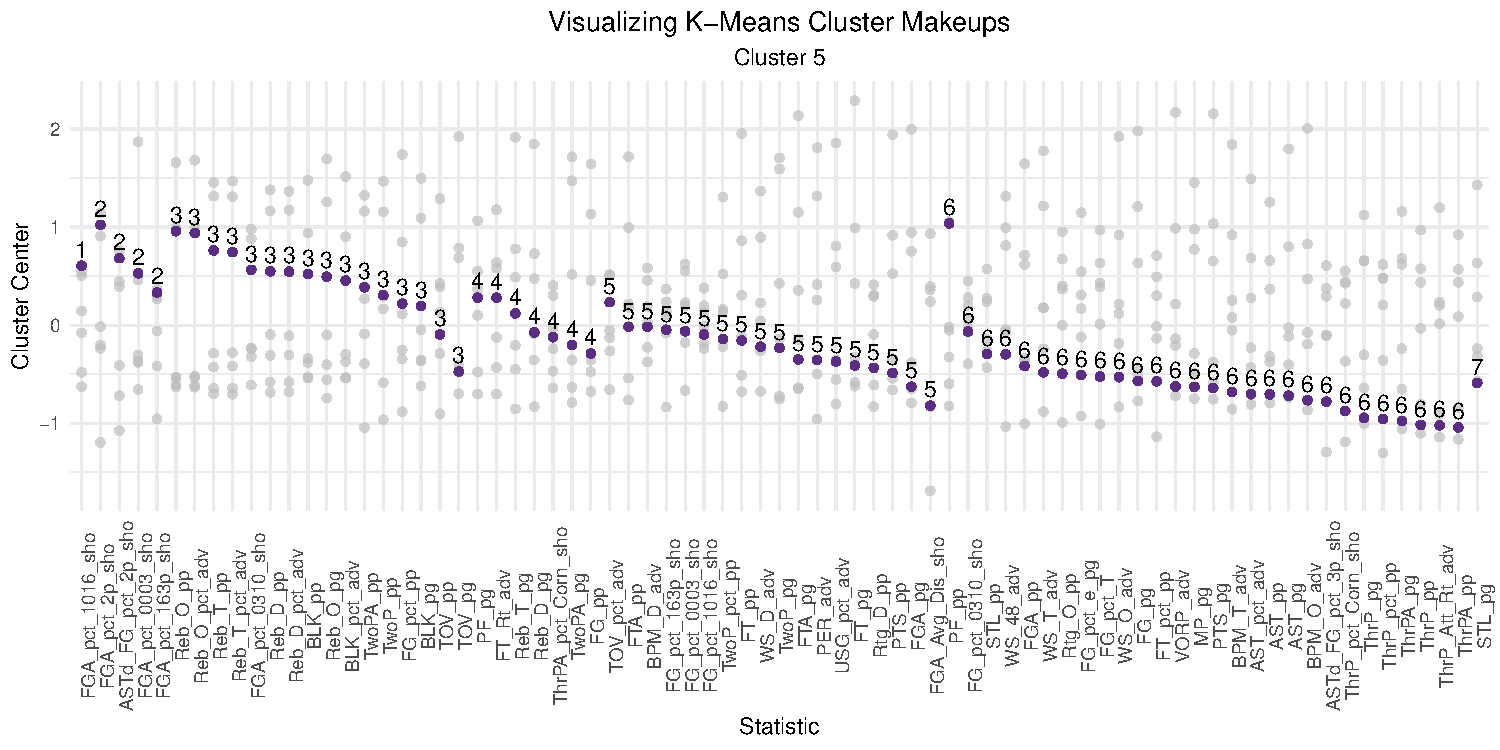
\includegraphics{Reclassifying-NBA-Player-Postions-Pt.-3---Clustering-Analysis-Results_files/figure-latex/unnamed-chunk-6-1.pdf}
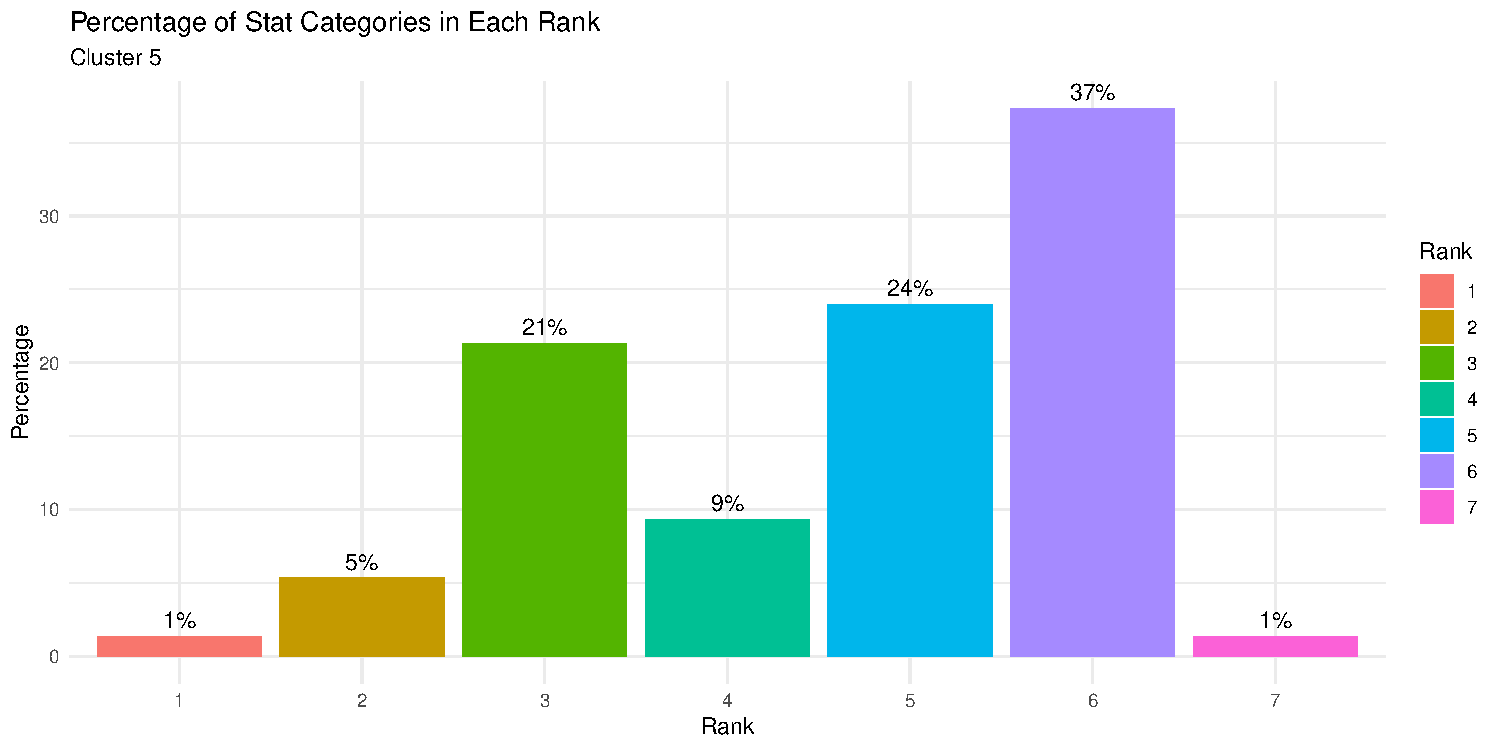
\includegraphics{Reclassifying-NBA-Player-Postions-Pt.-3---Clustering-Analysis-Results_files/figure-latex/unnamed-chunk-6-2.pdf}
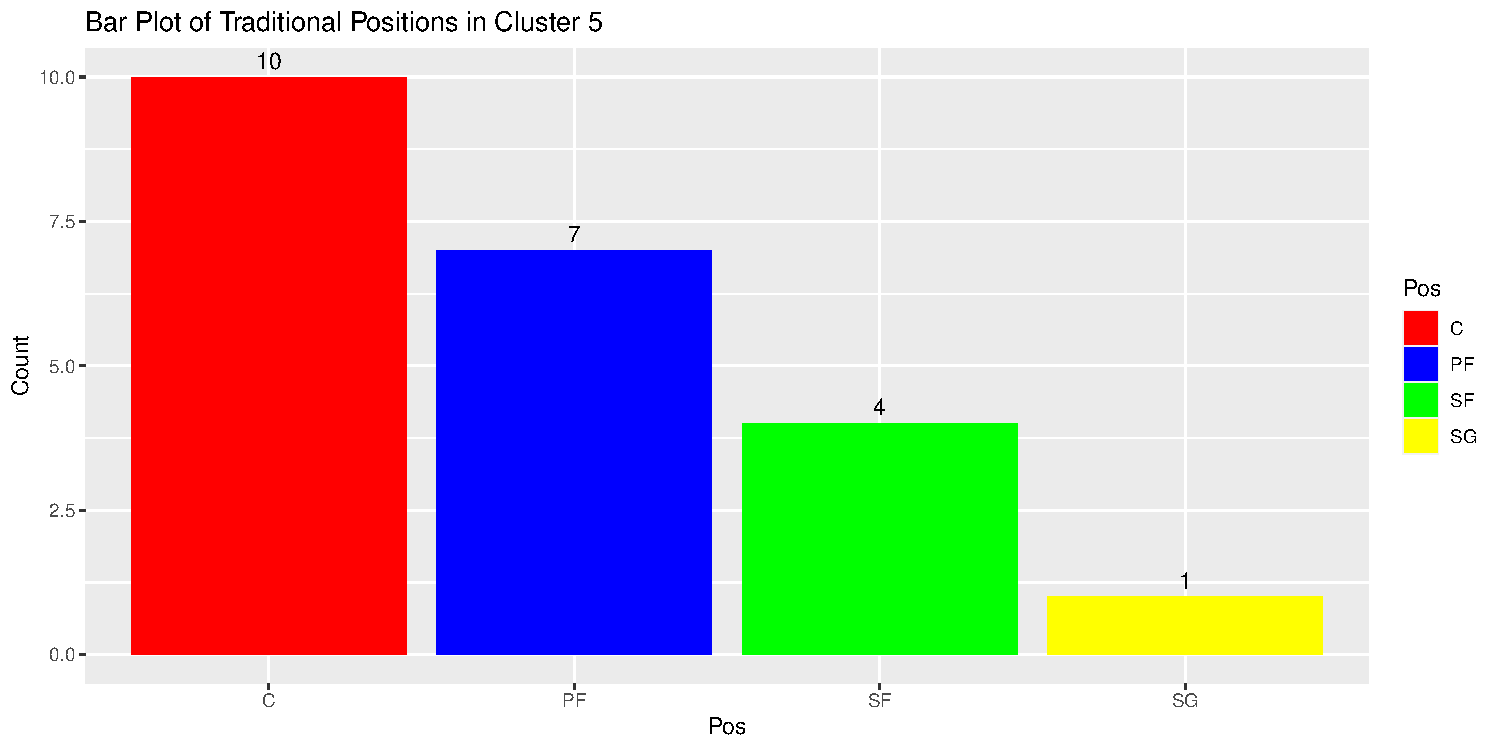
\includegraphics{Reclassifying-NBA-Player-Postions-Pt.-3---Clustering-Analysis-Results_files/figure-latex/unnamed-chunk-6-3.pdf}

\hypertarget{cluster-6}{%
\subsection{Cluster 6}\label{cluster-6}}

\begin{Shaded}
\begin{Highlighting}[]
\FunctionTok{cluster\_plots}\NormalTok{(}\StringTok{\textquotesingle{}Cluster 6\textquotesingle{}}\NormalTok{)}
\end{Highlighting}
\end{Shaded}

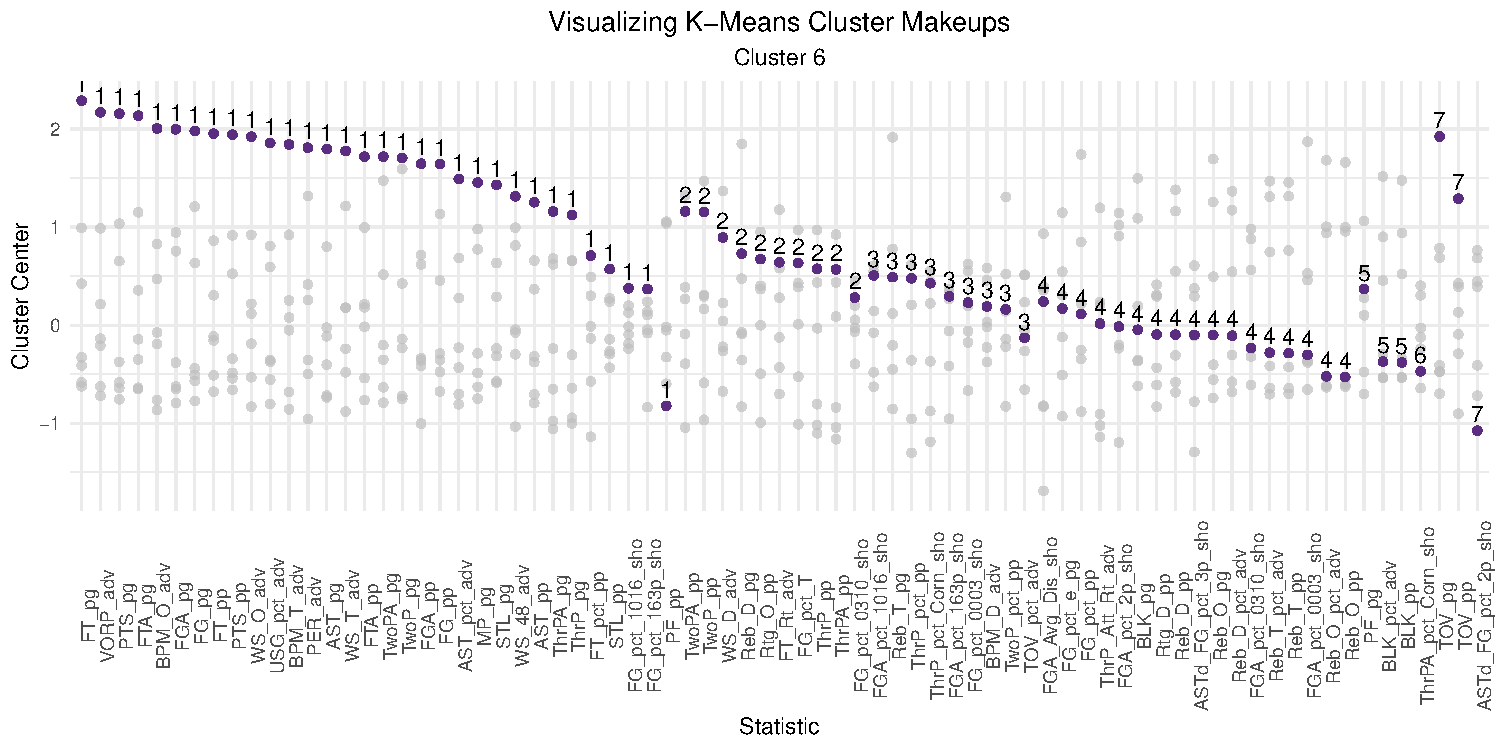
\includegraphics{Reclassifying-NBA-Player-Postions-Pt.-3---Clustering-Analysis-Results_files/figure-latex/unnamed-chunk-7-1.pdf}
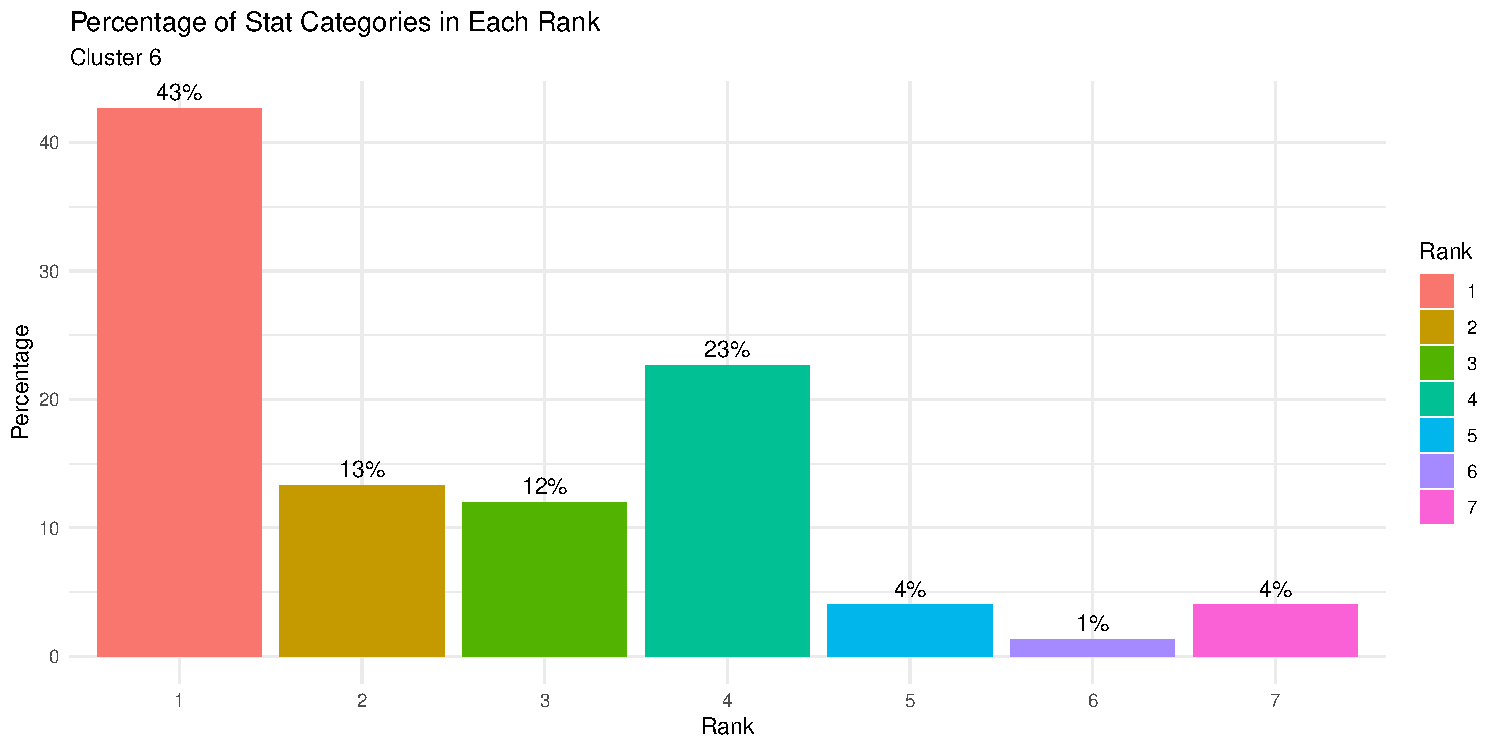
\includegraphics{Reclassifying-NBA-Player-Postions-Pt.-3---Clustering-Analysis-Results_files/figure-latex/unnamed-chunk-7-2.pdf}
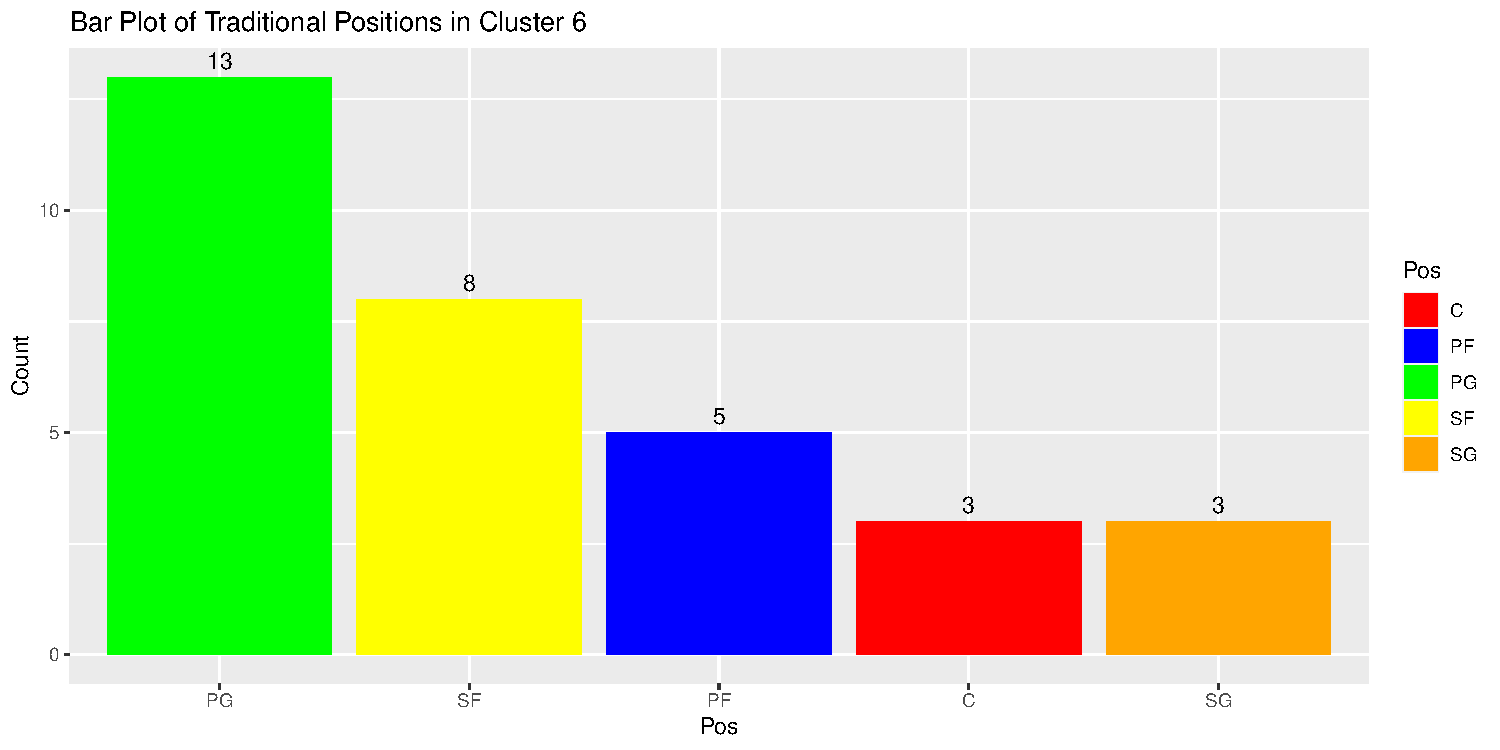
\includegraphics{Reclassifying-NBA-Player-Postions-Pt.-3---Clustering-Analysis-Results_files/figure-latex/unnamed-chunk-7-3.pdf}

\hypertarget{cluster-7}{%
\subsection{Cluster 7}\label{cluster-7}}

\begin{Shaded}
\begin{Highlighting}[]
\FunctionTok{cluster\_plots}\NormalTok{(}\StringTok{\textquotesingle{}Cluster 7\textquotesingle{}}\NormalTok{)}
\end{Highlighting}
\end{Shaded}

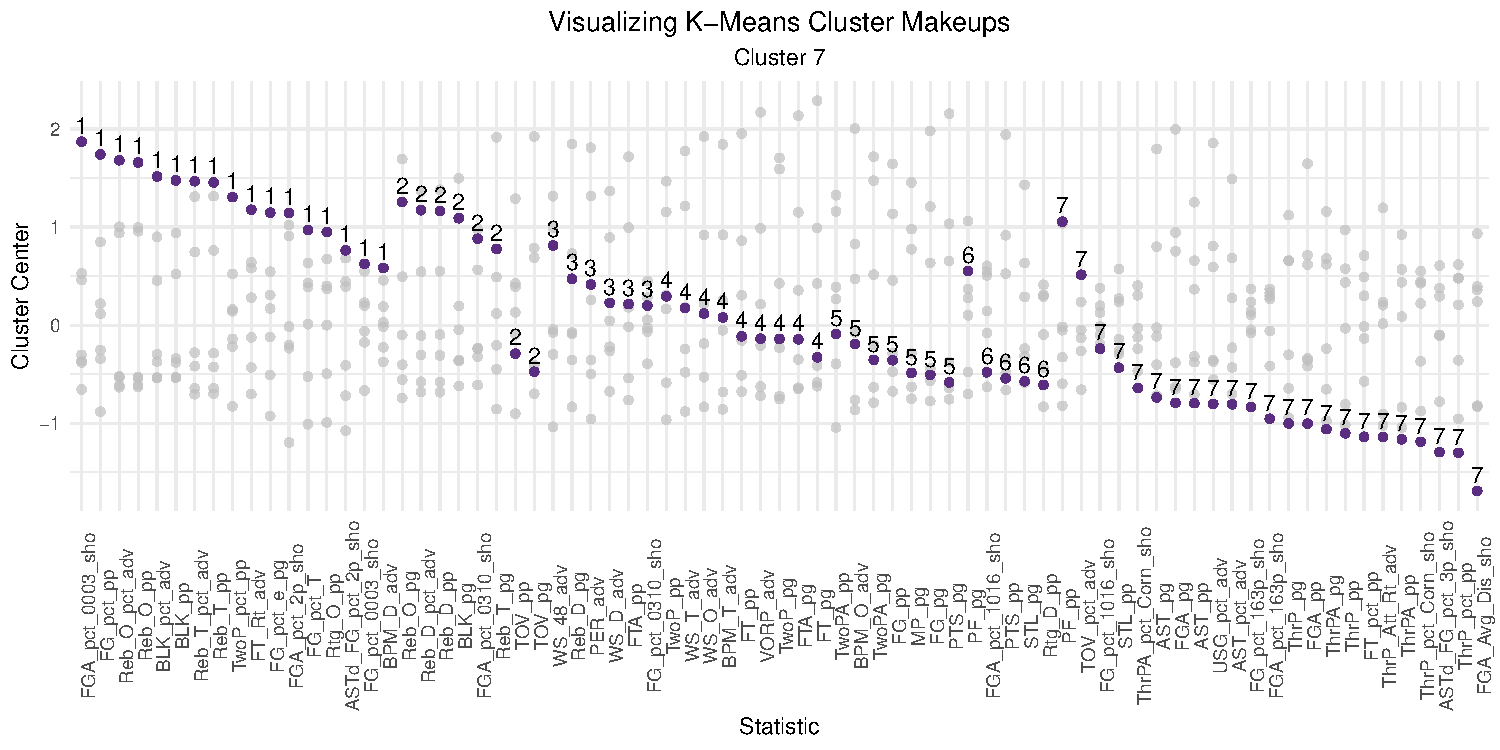
\includegraphics{Reclassifying-NBA-Player-Postions-Pt.-3---Clustering-Analysis-Results_files/figure-latex/unnamed-chunk-8-1.pdf}
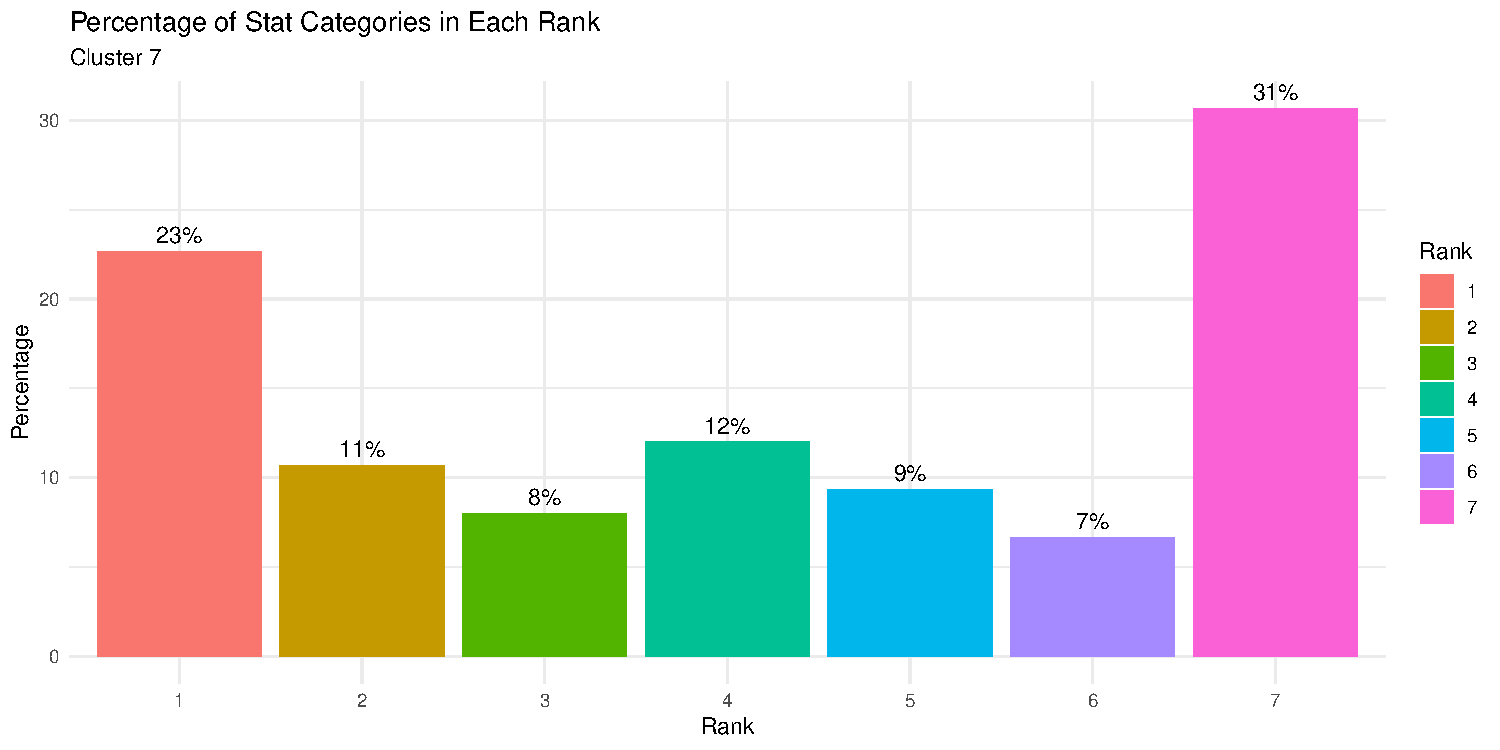
\includegraphics{Reclassifying-NBA-Player-Postions-Pt.-3---Clustering-Analysis-Results_files/figure-latex/unnamed-chunk-8-2.pdf}
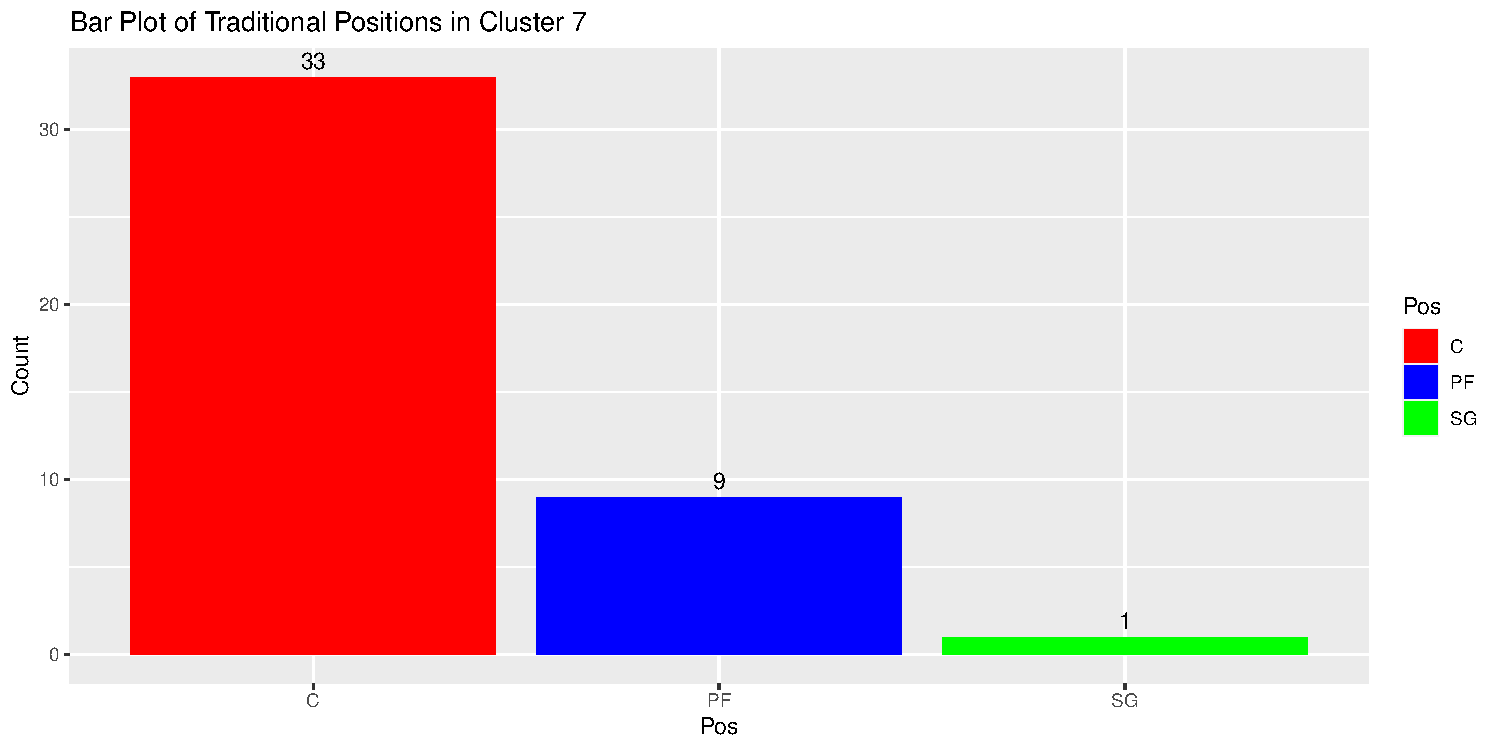
\includegraphics{Reclassifying-NBA-Player-Postions-Pt.-3---Clustering-Analysis-Results_files/figure-latex/unnamed-chunk-8-3.pdf}

\hypertarget{analysis-of-2022-players}{%
\section{Analysis of 2022 Players}\label{analysis-of-2022-players}}

\hypertarget{historical-and-current-cluster-analysis}{%
\subsection{Historical and Current Cluster
Analysis}\label{historical-and-current-cluster-analysis}}

The below plot shows how the player types have evolved since the
2000-2001 season and a brief summary of each cluster is included.

\begin{itemize}
\tightlist
\item
  MVP Bigs: Started to taper off in 2017. Went from about 8\%-11\% down
  to about 5\%-6\%. This position is most related to the traditional
  center role, which has significantly evolved over the years. More
  centers are taking threes and shooting the ball rather than playing in
  the post.
\item
  3-Point Backups: was generally between 17\% and 23\%, but then dropped
  to 12\% and 13\% in 2021 and 2022. Some of these players likely became
  3-Point Threats or Shooting Bigs in these years.
\item
  Game Generals: Fairly consistent over the years, ranging between
  16\%-24\% without any significant increases of decreases. It's
  actually the same in 2022 as it was in 2001 - 16\%
\item
  3-Point Threats: This position has shown the most dramatic increase -
  it was 6.4\% in 2004 and 41\% in 2022. The 3-point shot is a huge part
  of the game today.
\item
  Shooting Bigs: This position has shown the most dramatic decrease - it
  was 28\% in 2001 and fell to 2.5\% in 2020. A lot of these players
  have likely become 3-Point Threats.
\item
  Franchise Players: These players have always been part of the game,
  generally around 5\%-9\%.
\item
  Rebounding Bigs: These players have also generally been past of the
  game, ranging around 6\% to 13\%.
\end{itemize}

\begin{Shaded}
\begin{Highlighting}[]
\FunctionTok{ggplot}\NormalTok{(final\_df }\SpecialCharTok{\%\textgreater{}\%} \FunctionTok{mutate}\NormalTok{(}\AttributeTok{Year =} \FunctionTok{as.numeric}\NormalTok{(Year)),}
       \FunctionTok{aes}\NormalTok{(}\AttributeTok{x=}\NormalTok{Year, }
           \AttributeTok{fill=}\FunctionTok{factor}\NormalTok{(Cluster))}
\NormalTok{       ) }\SpecialCharTok{+}
  \FunctionTok{geom\_bar}\NormalTok{(}\AttributeTok{position=}\StringTok{"fill"}\NormalTok{) }\SpecialCharTok{+}
  \FunctionTok{geom\_text}\NormalTok{(}
    \FunctionTok{aes}\NormalTok{(}\AttributeTok{label=}\FunctionTok{paste0}\NormalTok{(}\FunctionTok{signif}\NormalTok{(..count.. }\SpecialCharTok{/} \FunctionTok{tapply}\NormalTok{(..count.., ..x.., sum)[}\FunctionTok{as.character}\NormalTok{(..x..)]}\SpecialCharTok{*}\DecValTok{100}\NormalTok{, }\AttributeTok{digits=}\DecValTok{2}\NormalTok{),}\StringTok{"\%"}\NormalTok{)), }
    \AttributeTok{stat=}\StringTok{"count"}\NormalTok{,}
    \AttributeTok{position=}\FunctionTok{position\_fill}\NormalTok{(}\AttributeTok{vjust=}\FloatTok{0.5}\NormalTok{),}\AttributeTok{colour=}\StringTok{"black"}\NormalTok{, }\AttributeTok{size=}\DecValTok{3}\NormalTok{)}\SpecialCharTok{+}
  \FunctionTok{labs}\NormalTok{(}\AttributeTok{y=}\StringTok{"Percentage"}\NormalTok{) }\SpecialCharTok{+}
  \FunctionTok{scale\_x\_continuous}\NormalTok{(}\StringTok{"Year"}\NormalTok{, }\AttributeTok{breaks=}\FunctionTok{seq}\NormalTok{(}\DecValTok{2001}\NormalTok{,}\DecValTok{2022}\NormalTok{,}\AttributeTok{by=}\DecValTok{1}\NormalTok{)) }\SpecialCharTok{+}
  \FunctionTok{scale\_y\_continuous}\NormalTok{(}\AttributeTok{labels =}\NormalTok{ scales}\SpecialCharTok{::}\FunctionTok{percent\_format}\NormalTok{(}\AttributeTok{accuracy =} \DecValTok{1}\NormalTok{)) }\SpecialCharTok{+}
  \FunctionTok{theme}\NormalTok{(}\AttributeTok{axis.text.x =} \FunctionTok{element\_text}\NormalTok{(}\AttributeTok{angle =} \DecValTok{90}\NormalTok{, }\AttributeTok{vjust =} \FloatTok{0.5}\NormalTok{, }\AttributeTok{hjust=}\DecValTok{1}\NormalTok{)) }\SpecialCharTok{+}
  \FunctionTok{scale\_fill\_discrete}\NormalTok{(}\AttributeTok{name =} \StringTok{"Player}\SpecialCharTok{\textbackslash{}n}\StringTok{Type"}\NormalTok{, }\AttributeTok{labels =}\FunctionTok{c}\NormalTok{(}\StringTok{\textquotesingle{}MVP Bigs\textquotesingle{}}\NormalTok{, }\StringTok{\textquotesingle{}3{-}Point}\SpecialCharTok{\textbackslash{}n}\StringTok{Backups\textquotesingle{}}\NormalTok{, }\StringTok{\textquotesingle{}Game}\SpecialCharTok{\textbackslash{}n}\StringTok{Generals\textquotesingle{}}\NormalTok{, }\StringTok{\textquotesingle{}3{-}Point}\SpecialCharTok{\textbackslash{}n}\StringTok{Threats\textquotesingle{}}\NormalTok{,}\StringTok{\textquotesingle{}Shooting}\SpecialCharTok{\textbackslash{}n}\StringTok{Bigs\textquotesingle{}}\NormalTok{, }\StringTok{\textquotesingle{}Franchise}\SpecialCharTok{\textbackslash{}n}\StringTok{Players\textquotesingle{}}\NormalTok{, }\StringTok{\textquotesingle{}Rebounding}\SpecialCharTok{\textbackslash{}n}\StringTok{Bigs\textquotesingle{}}\NormalTok{)) }\SpecialCharTok{+}
  \FunctionTok{theme}\NormalTok{(}\AttributeTok{legend.key.height=}\FunctionTok{unit}\NormalTok{(}\DecValTok{1}\NormalTok{, }\StringTok{"cm"}\NormalTok{))}
\end{Highlighting}
\end{Shaded}

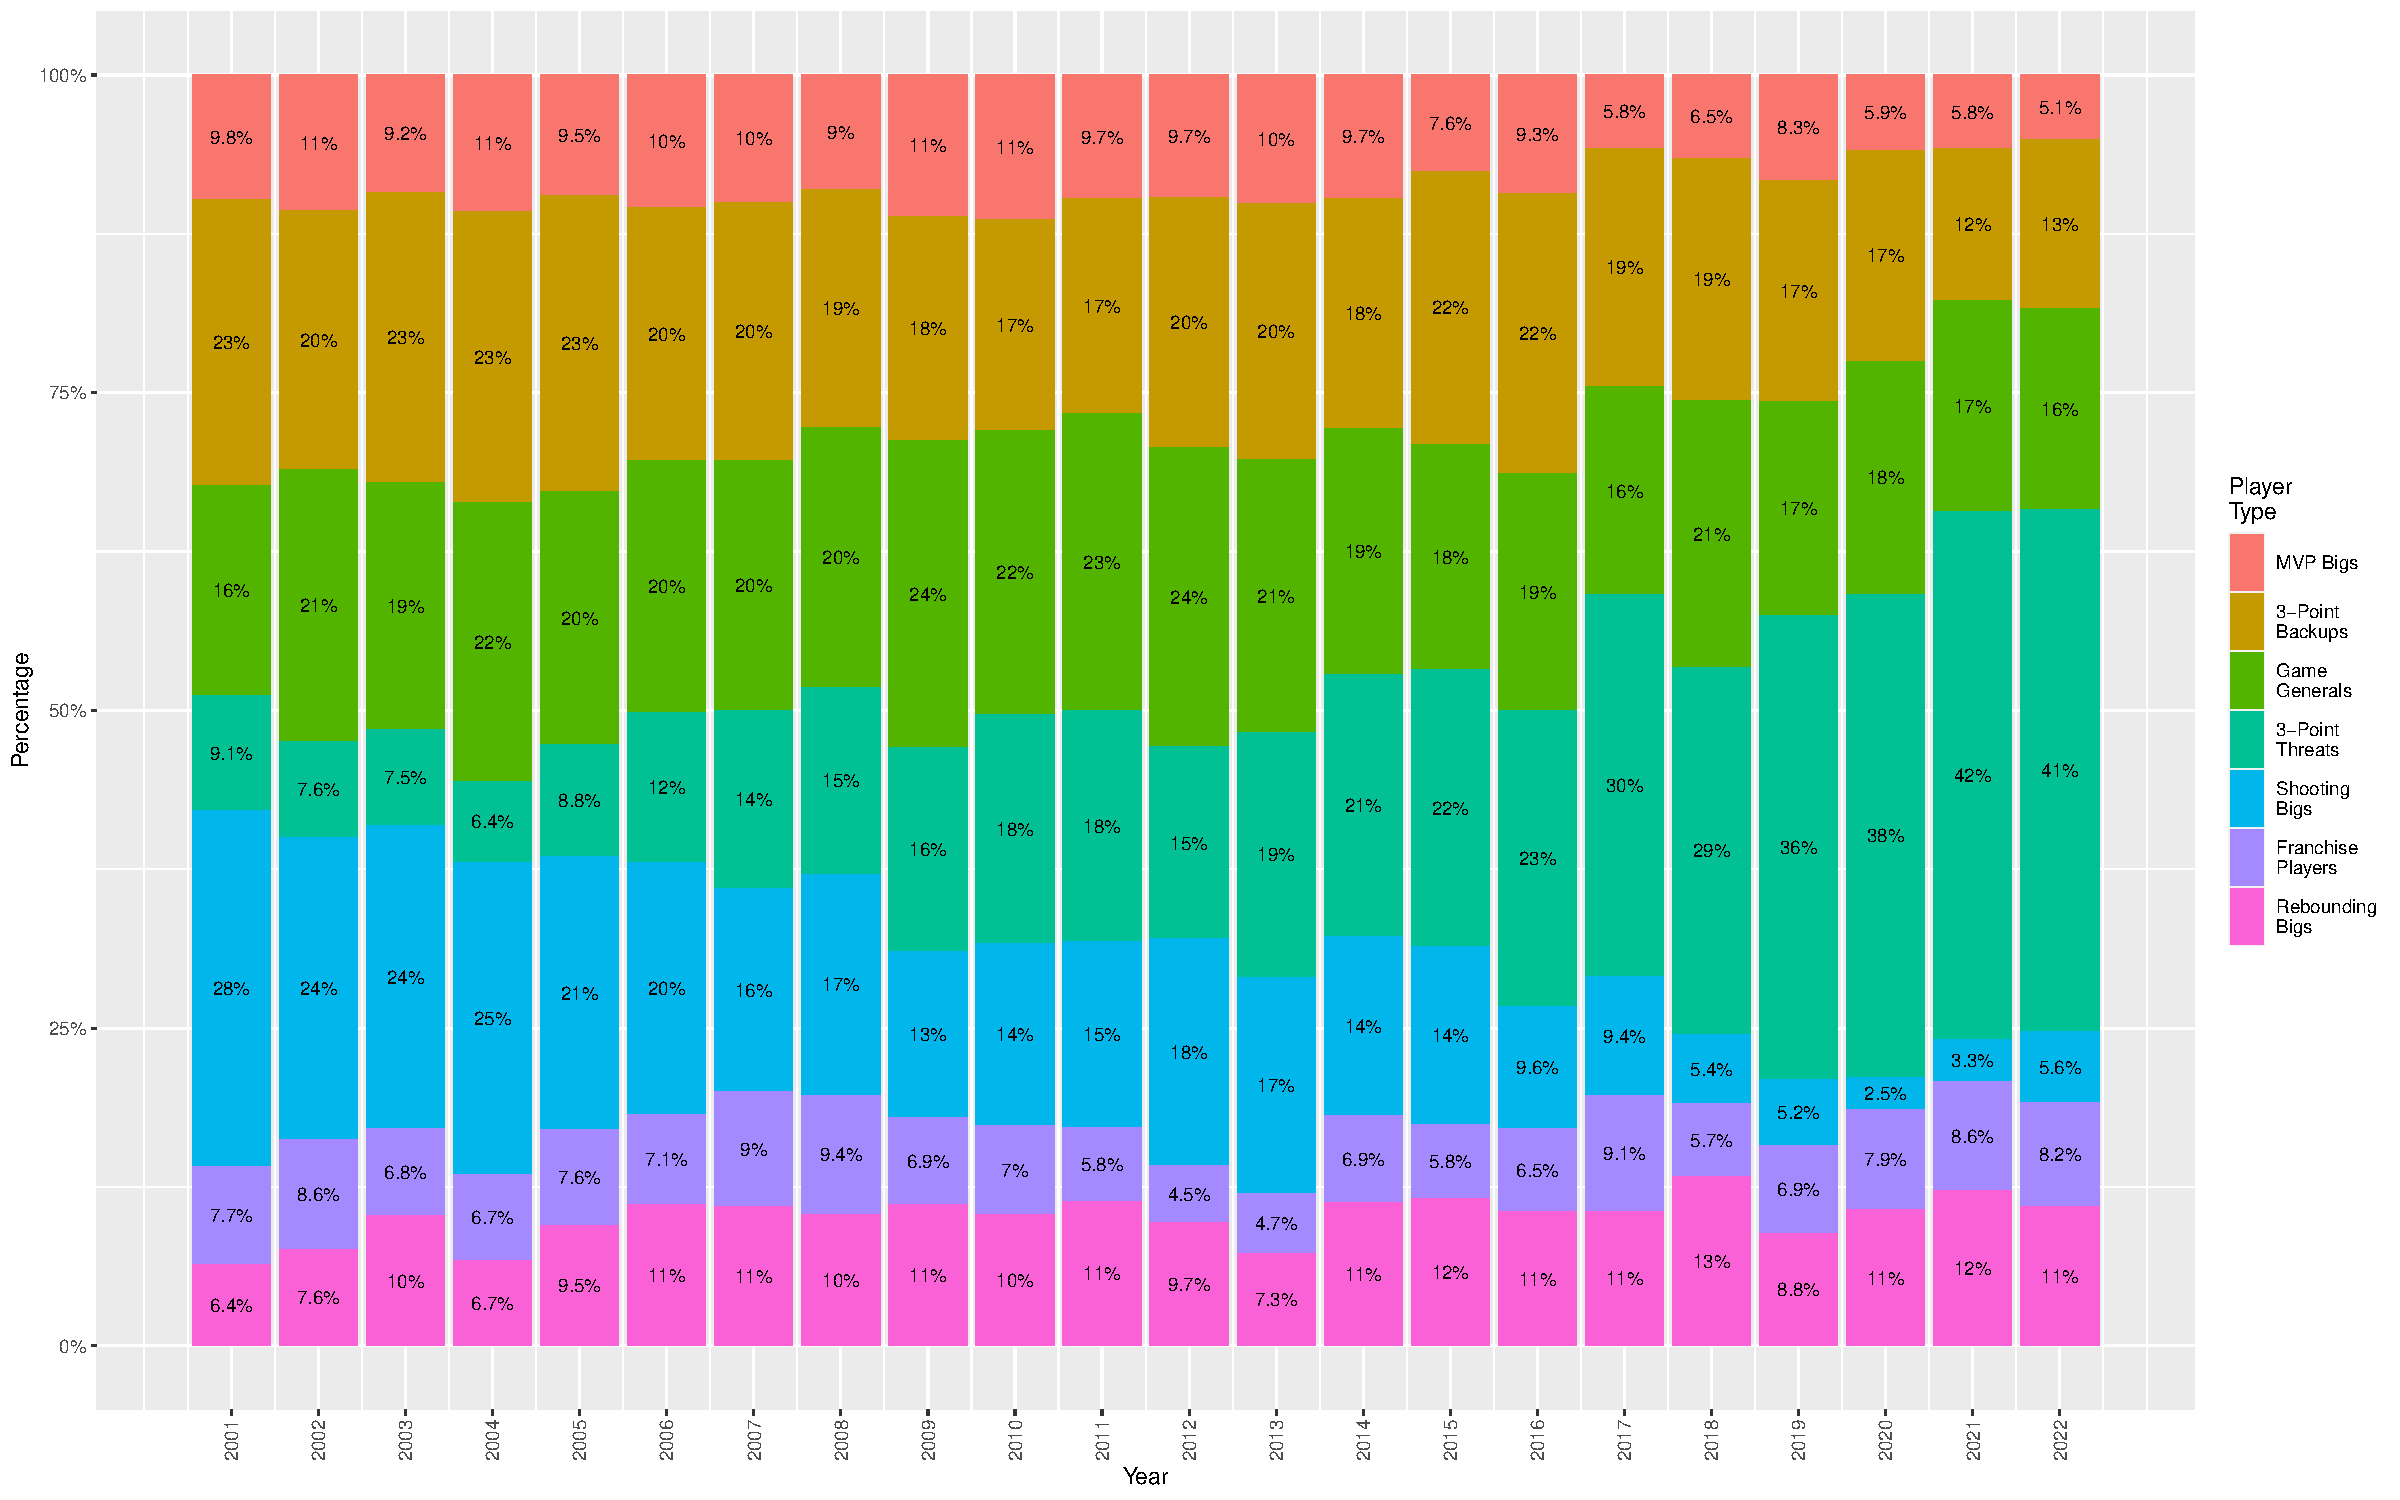
\includegraphics{Reclassifying-NBA-Player-Postions-Pt.-3---Clustering-Analysis-Results_files/figure-latex/unnamed-chunk-10-1.pdf}

\hypertarget{count-of-traditional-position-in-each-new-player-type---2022}{%
\subsection{Count of Traditional Position in Each New Player Type -
2022}\label{count-of-traditional-position-in-each-new-player-type---2022}}

The plot below displays the count of each traditional player position
(C, PF, SF, SG, PG) within each of the new clusters (i.e.~new player
types).

\begin{enumerate}
\def\labelenumi{\arabic{enumi}.}
\tightlist
\item
  MVP Bigs
\item
  3-point Backups
\item
  Game Generals
\item
  3-point Threats
\item
  Shooting Bigs
\item
  Franchise Players
\item
  Rebounding Bigs
\end{enumerate}

\begin{itemize}
\tightlist
\item
  Of the seven new player types, four have players from each traditional
  position - 3-point Backups, Game Generals, 3-point Threats, and
  Franchise Players. However, 3-point Backups and Game Generals only
  have 1 center each.
\item
  MVP Bigs and Rebounding Bigs only have Power Forwards and Centers with
  the exception of Rebounding Bigs, which includes one shooting guard.
\end{itemize}

\begin{Shaded}
\begin{Highlighting}[]
\FunctionTok{ggplot}\NormalTok{(final\_df }\SpecialCharTok{\%\textgreater{}\%} 
         \FunctionTok{mutate}\NormalTok{(}\AttributeTok{Year =} \FunctionTok{as.numeric}\NormalTok{(Year),}
                \AttributeTok{Cluster =} \FunctionTok{as.numeric}\NormalTok{(Cluster)) }\SpecialCharTok{\%\textgreater{}\%}
         \FunctionTok{filter}\NormalTok{(Year }\SpecialCharTok{==} \DecValTok{2022}\NormalTok{),}
       \FunctionTok{aes}\NormalTok{(}\AttributeTok{x =}\NormalTok{ Cluster, }\AttributeTok{fill =}\NormalTok{ Pos)) }\SpecialCharTok{+}
  \FunctionTok{geom\_bar}\NormalTok{(}\FunctionTok{aes}\NormalTok{(}\AttributeTok{y =}\NormalTok{ (..count..)),}\AttributeTok{colour=}\StringTok{"white"}\NormalTok{) }\SpecialCharTok{+}
  \FunctionTok{geom\_text}\NormalTok{(}\AttributeTok{stat=}\StringTok{\textquotesingle{}count\textquotesingle{}}\NormalTok{, }\FunctionTok{aes}\NormalTok{(}\AttributeTok{label=}\NormalTok{..count..),}\AttributeTok{position =} \FunctionTok{position\_stack}\NormalTok{(}\AttributeTok{vjust =} \FloatTok{0.5}\NormalTok{), }\AttributeTok{color =} \StringTok{"black"}\NormalTok{) }\SpecialCharTok{+}
  \FunctionTok{ggtitle}\NormalTok{(}\StringTok{"Count of Traditional Position in Each New Player Type {-} 2022"}\NormalTok{) }\SpecialCharTok{+}
  \FunctionTok{theme}\NormalTok{(}\AttributeTok{plot.title =} \FunctionTok{element\_text}\NormalTok{(}\AttributeTok{hjust =} \FloatTok{0.5}\NormalTok{)) }\SpecialCharTok{+}
  \FunctionTok{scale\_x\_continuous}\NormalTok{(}\AttributeTok{name =} \StringTok{"New Position Name"}\NormalTok{, }\AttributeTok{breaks =} \FunctionTok{c}\NormalTok{(}\DecValTok{1}\NormalTok{, }\DecValTok{2}\NormalTok{, }\DecValTok{3}\NormalTok{, }\DecValTok{4}\NormalTok{, }\DecValTok{5}\NormalTok{, }\DecValTok{6}\NormalTok{, }\DecValTok{7}\NormalTok{),}
                     \AttributeTok{labels =} \FunctionTok{c}\NormalTok{(}\StringTok{\textquotesingle{}MVP Bigs\textquotesingle{}}\NormalTok{, }\StringTok{\textquotesingle{}3{-}Point}\SpecialCharTok{\textbackslash{}n}\StringTok{Backups\textquotesingle{}}\NormalTok{, }\StringTok{\textquotesingle{}Game}\SpecialCharTok{\textbackslash{}n}\StringTok{Generals\textquotesingle{}}\NormalTok{, }\StringTok{\textquotesingle{}3{-}Point}\SpecialCharTok{\textbackslash{}n}\StringTok{Threats\textquotesingle{}}\NormalTok{, }\StringTok{\textquotesingle{}Shooting}\SpecialCharTok{\textbackslash{}n}\StringTok{Bigs\textquotesingle{}}\NormalTok{, }\StringTok{\textquotesingle{}Franchise}\SpecialCharTok{\textbackslash{}n}\StringTok{Players\textquotesingle{}}\NormalTok{, }\StringTok{\textquotesingle{}Rebounding}\SpecialCharTok{\textbackslash{}n}\StringTok{Bigs\textquotesingle{}}\NormalTok{)) }\SpecialCharTok{+}
  \FunctionTok{labs}\NormalTok{(}\AttributeTok{fill =} \StringTok{"Traditional Position"}\NormalTok{, }\AttributeTok{y =} \StringTok{"Count"}\NormalTok{) }\SpecialCharTok{+}
  \FunctionTok{theme}\NormalTok{(}\AttributeTok{legend.key.height=}\FunctionTok{unit}\NormalTok{(}\DecValTok{2}\NormalTok{, }\StringTok{"cm"}\NormalTok{))}
\end{Highlighting}
\end{Shaded}

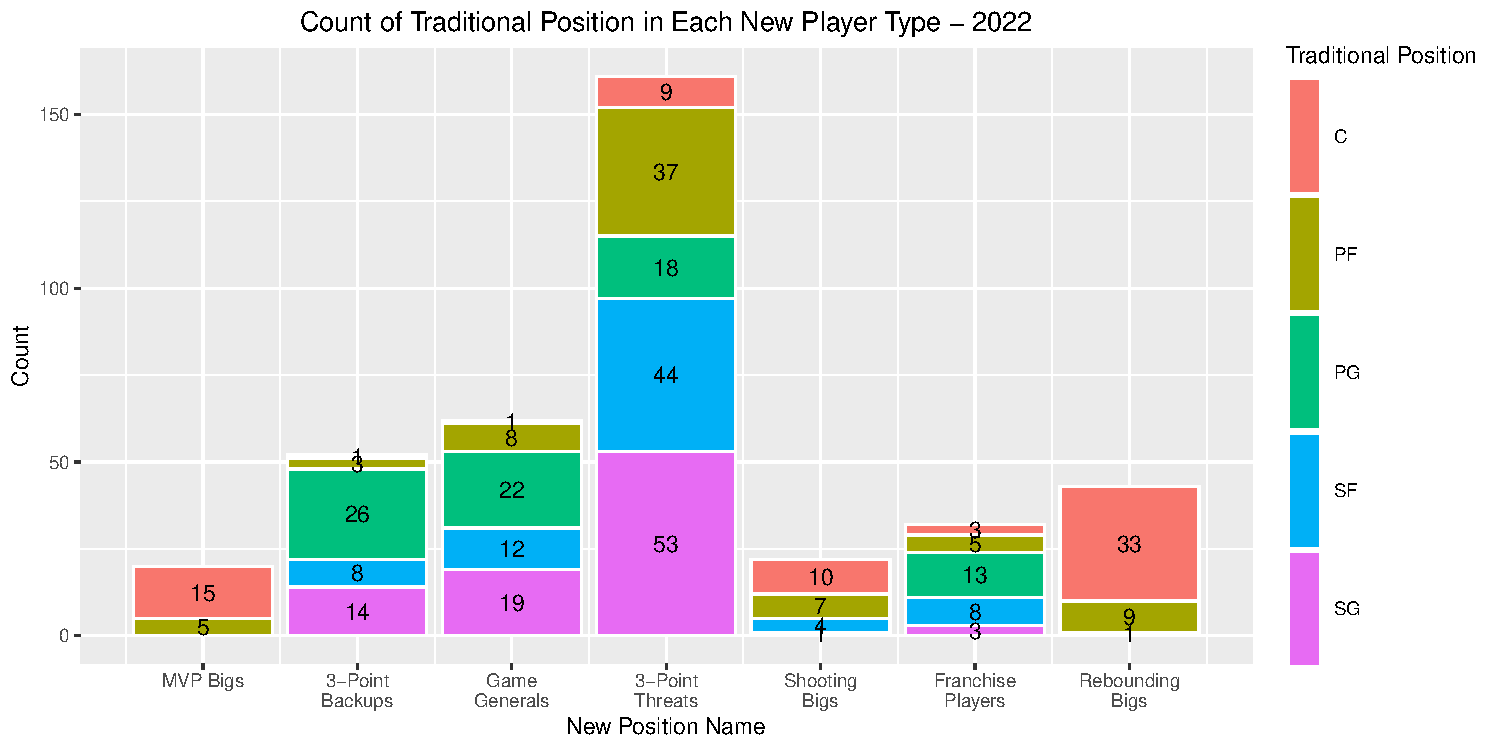
\includegraphics{Reclassifying-NBA-Player-Postions-Pt.-3---Clustering-Analysis-Results_files/figure-latex/unnamed-chunk-11-1.pdf}

\hypertarget{percentage-of-cluster-within-each-traditional-position---2022}{%
\subsection{Percentage of Cluster within Each Traditional Position -
2022}\label{percentage-of-cluster-within-each-traditional-position---2022}}

\begin{Shaded}
\begin{Highlighting}[]
\NormalTok{dat }\OtherTok{\textless{}{-}}\NormalTok{ final\_df }\SpecialCharTok{\%\textgreater{}\%} \FunctionTok{filter}\NormalTok{(Year }\SpecialCharTok{==}\DecValTok{2022}\NormalTok{) }
\NormalTok{dat1 }\OtherTok{\textless{}{-}} \FunctionTok{as.data.frame}\NormalTok{(}\FunctionTok{prop.table}\NormalTok{(}\FunctionTok{table}\NormalTok{(dat}\SpecialCharTok{$}\NormalTok{Pos, dat}\SpecialCharTok{$}\NormalTok{Cluster), }\AttributeTok{margin =} \DecValTok{1}\NormalTok{))}
\FunctionTok{colnames}\NormalTok{(dat1) }\OtherTok{\textless{}{-}} \FunctionTok{c}\NormalTok{(}\StringTok{"Pos"}\NormalTok{, }\StringTok{"Cluster"}\NormalTok{, }\StringTok{"percent"}\NormalTok{)}

\NormalTok{dat1 }\OtherTok{\textless{}{-}}\NormalTok{ dat1 }\SpecialCharTok{\%\textgreater{}\%} 
  \FunctionTok{group\_by}\NormalTok{(Pos) }\SpecialCharTok{\%\textgreater{}\%} 
  \FunctionTok{mutate}\NormalTok{(}\AttributeTok{Pos\_label\_y =} \DecValTok{1} \SpecialCharTok{{-}}\NormalTok{ (}\FunctionTok{cumsum}\NormalTok{(percent) }\SpecialCharTok{{-}} \FloatTok{0.5} \SpecialCharTok{*}\NormalTok{ percent)) }\SpecialCharTok{\%\textgreater{}\%} 
  \FunctionTok{ungroup}\NormalTok{()}

\FunctionTok{ggplot}\NormalTok{(dat1, }\FunctionTok{aes}\NormalTok{(Pos, }\AttributeTok{y =}\NormalTok{ percent, }\AttributeTok{fill =} \FunctionTok{factor}\NormalTok{(Cluster))) }\SpecialCharTok{+}
  \FunctionTok{geom\_bar}\NormalTok{(}\AttributeTok{data =}\NormalTok{ . }\SpecialCharTok{\%\textgreater{}\%} \FunctionTok{filter}\NormalTok{(percent }\SpecialCharTok{\textgreater{}} \DecValTok{0}\NormalTok{), }\AttributeTok{position =} \StringTok{"fill"}\NormalTok{, }\AttributeTok{stat =} \StringTok{"identity"}\NormalTok{) }\SpecialCharTok{+}
  \FunctionTok{scale\_y\_continuous}\NormalTok{(}\AttributeTok{labels =}\NormalTok{ scales}\SpecialCharTok{::}\NormalTok{percent) }\SpecialCharTok{+}
  \FunctionTok{geom\_text}\NormalTok{(}\AttributeTok{data =}\NormalTok{ . }\SpecialCharTok{\%\textgreater{}\%} \FunctionTok{filter}\NormalTok{(percent }\SpecialCharTok{\textgreater{}} \DecValTok{0}\NormalTok{), }\FunctionTok{aes}\NormalTok{(}\AttributeTok{y =}\NormalTok{ Pos\_label\_y, }\AttributeTok{label =} \FunctionTok{round}\NormalTok{(}\DecValTok{100} \SpecialCharTok{*}\NormalTok{ percent, }\DecValTok{1}\NormalTok{))) }\SpecialCharTok{+}
  \FunctionTok{ggtitle}\NormalTok{(}\StringTok{"Percentage of Cluster within Each Traditional Position {-} 2022"}\NormalTok{) }\SpecialCharTok{+}
  \FunctionTok{theme}\NormalTok{(}\AttributeTok{plot.title =} \FunctionTok{element\_text}\NormalTok{(}\AttributeTok{hjust =} \FloatTok{0.5}\NormalTok{)) }\SpecialCharTok{+}
  \FunctionTok{scale\_x\_discrete}\NormalTok{(}\AttributeTok{name =} \StringTok{"Traditional Position"}\NormalTok{) }\SpecialCharTok{+}
  \FunctionTok{scale\_fill\_discrete}\NormalTok{(}\AttributeTok{name =} \StringTok{"New Position Name"}\NormalTok{, }\AttributeTok{labels =} \FunctionTok{c}\NormalTok{(}\StringTok{\textquotesingle{}MVP Bigs\textquotesingle{}}\NormalTok{, }\StringTok{\textquotesingle{}3{-}Point}\SpecialCharTok{\textbackslash{}n}\StringTok{Backups\textquotesingle{}}\NormalTok{, }\StringTok{\textquotesingle{}Game}\SpecialCharTok{\textbackslash{}n}\StringTok{Generals\textquotesingle{}}\NormalTok{, }\StringTok{\textquotesingle{}3{-}Point}\SpecialCharTok{\textbackslash{}n}\StringTok{Threats\textquotesingle{}}\NormalTok{, }\StringTok{\textquotesingle{}Shooting}\SpecialCharTok{\textbackslash{}n}\StringTok{Bigs\textquotesingle{}}\NormalTok{, }\StringTok{\textquotesingle{}Franchise}\SpecialCharTok{\textbackslash{}n}\StringTok{Players\textquotesingle{}}\NormalTok{, }\StringTok{\textquotesingle{}Rebounding}\SpecialCharTok{\textbackslash{}n}\StringTok{Bigs\textquotesingle{}}\NormalTok{)) }\SpecialCharTok{+}
  \FunctionTok{ylab}\NormalTok{(}\StringTok{"Percentage"}\NormalTok{) }\SpecialCharTok{+}
  \FunctionTok{theme}\NormalTok{(}\AttributeTok{strip.background =} \FunctionTok{element\_blank}\NormalTok{(),}
        \AttributeTok{strip.text =} \FunctionTok{element\_blank}\NormalTok{(),}
        \AttributeTok{legend.key.height =} \FunctionTok{unit}\NormalTok{(}\DecValTok{1}\NormalTok{, }\StringTok{"cm"}\NormalTok{))}
\end{Highlighting}
\end{Shaded}

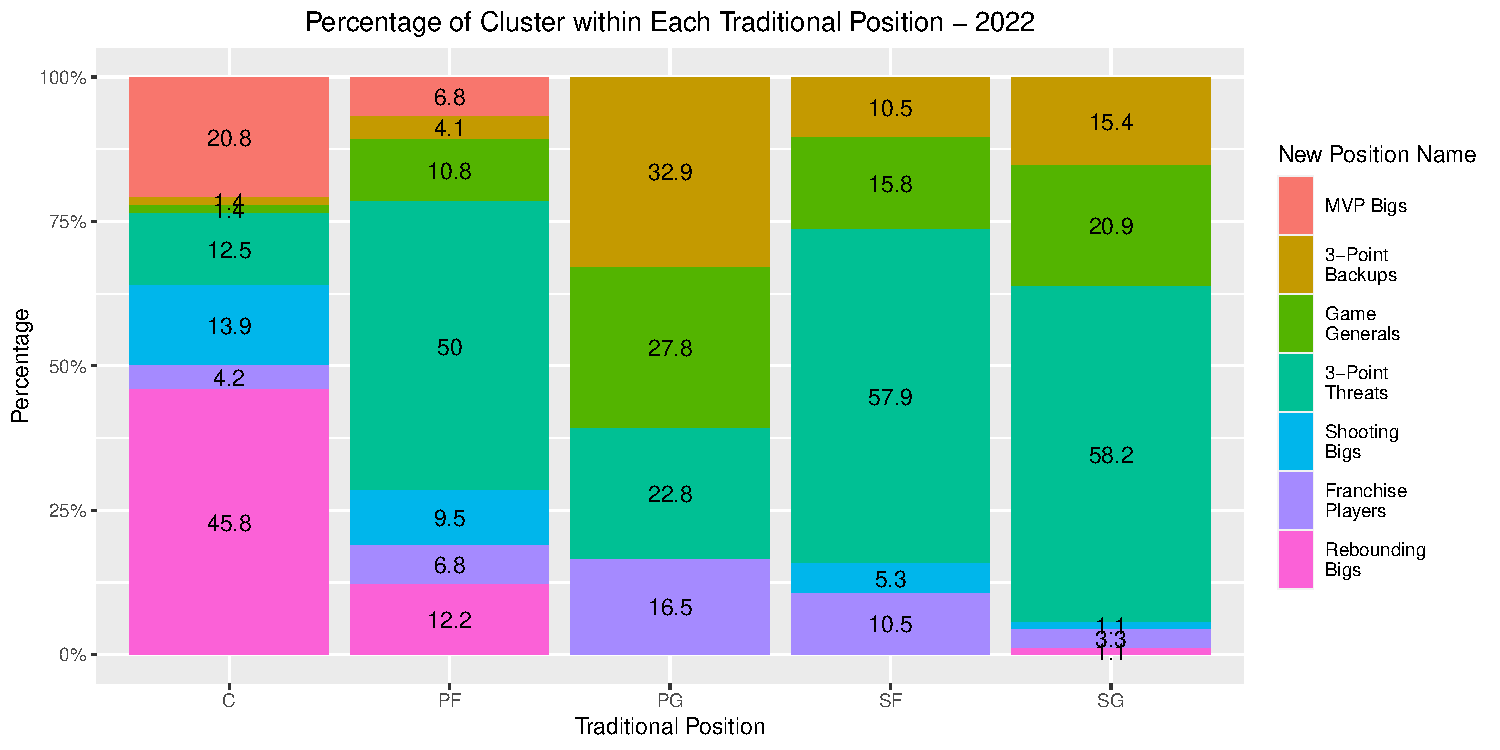
\includegraphics{Reclassifying-NBA-Player-Postions-Pt.-3---Clustering-Analysis-Results_files/figure-latex/unnamed-chunk-12-1.pdf}

\hypertarget{count-of-new-position-on-each-team---2022}{%
\subsection{Count of New Position on Each Team -
2022}\label{count-of-new-position-on-each-team---2022}}

\begin{Shaded}
\begin{Highlighting}[]
\CommentTok{\#teams by cluster}
\FunctionTok{ggplot}\NormalTok{(df\_2022 }\SpecialCharTok{\%\textgreater{}\%} 
         \FunctionTok{mutate}\NormalTok{(}\AttributeTok{Year =} \FunctionTok{as.numeric}\NormalTok{(Year),}
                \AttributeTok{Cluster =} \FunctionTok{as.numeric}\NormalTok{(Cluster)) }\SpecialCharTok{\%\textgreater{}\%}
         \FunctionTok{filter}\NormalTok{(Year }\SpecialCharTok{==} \DecValTok{2022}\NormalTok{),}
       \FunctionTok{aes}\NormalTok{(}\AttributeTok{x =}\NormalTok{ Tm, }\AttributeTok{fill =} \FunctionTok{factor}\NormalTok{(Cluster))) }\SpecialCharTok{+}
  \FunctionTok{ggtitle}\NormalTok{(}\StringTok{"Count of New Position on Each Team {-} 2022"}\NormalTok{) }\SpecialCharTok{+}
  \FunctionTok{geom\_bar}\NormalTok{(}\AttributeTok{position =} \StringTok{"fill"}\NormalTok{) }\SpecialCharTok{+} \FunctionTok{ylab}\NormalTok{(}\StringTok{"Proportion"}\NormalTok{) }\SpecialCharTok{+}
  \FunctionTok{stat\_count}\NormalTok{(}\AttributeTok{geom =} \StringTok{"text"}\NormalTok{, }
             \FunctionTok{aes}\NormalTok{(}\AttributeTok{label =} \FunctionTok{stat}\NormalTok{(count)),}
             \AttributeTok{position=}\FunctionTok{position\_fill}\NormalTok{(}\AttributeTok{vjust=}\FloatTok{0.5}\NormalTok{), }\AttributeTok{colour=}\StringTok{"white"}\NormalTok{) }\SpecialCharTok{+}
    \FunctionTok{scale\_fill\_discrete}\NormalTok{(}\AttributeTok{name =} \StringTok{"New Position"}\NormalTok{, }\AttributeTok{labels =}\FunctionTok{c}\NormalTok{(}\StringTok{\textquotesingle{}MVP Bigs\textquotesingle{}}\NormalTok{, }\StringTok{\textquotesingle{}3{-}Point}\SpecialCharTok{\textbackslash{}n}\StringTok{Backups\textquotesingle{}}\NormalTok{, }\StringTok{\textquotesingle{}Game}\SpecialCharTok{\textbackslash{}n}\StringTok{Generals\textquotesingle{}}\NormalTok{, }\StringTok{\textquotesingle{}3{-}Point}\SpecialCharTok{\textbackslash{}n}\StringTok{Threats\textquotesingle{}}\NormalTok{, }\StringTok{\textquotesingle{}Shooting}\SpecialCharTok{\textbackslash{}n}\StringTok{Bigs\textquotesingle{}}\NormalTok{, }\StringTok{\textquotesingle{}Franchise}\SpecialCharTok{\textbackslash{}n}\StringTok{Players\textquotesingle{}}\NormalTok{, }\StringTok{\textquotesingle{}Rebounding}\SpecialCharTok{\textbackslash{}n}\StringTok{Bigs\textquotesingle{}}\NormalTok{)) }\SpecialCharTok{+}
  \FunctionTok{theme}\NormalTok{(}\AttributeTok{legend.key.height=}\FunctionTok{unit}\NormalTok{(}\DecValTok{1}\NormalTok{, }\StringTok{"cm"}\NormalTok{))}
\end{Highlighting}
\end{Shaded}

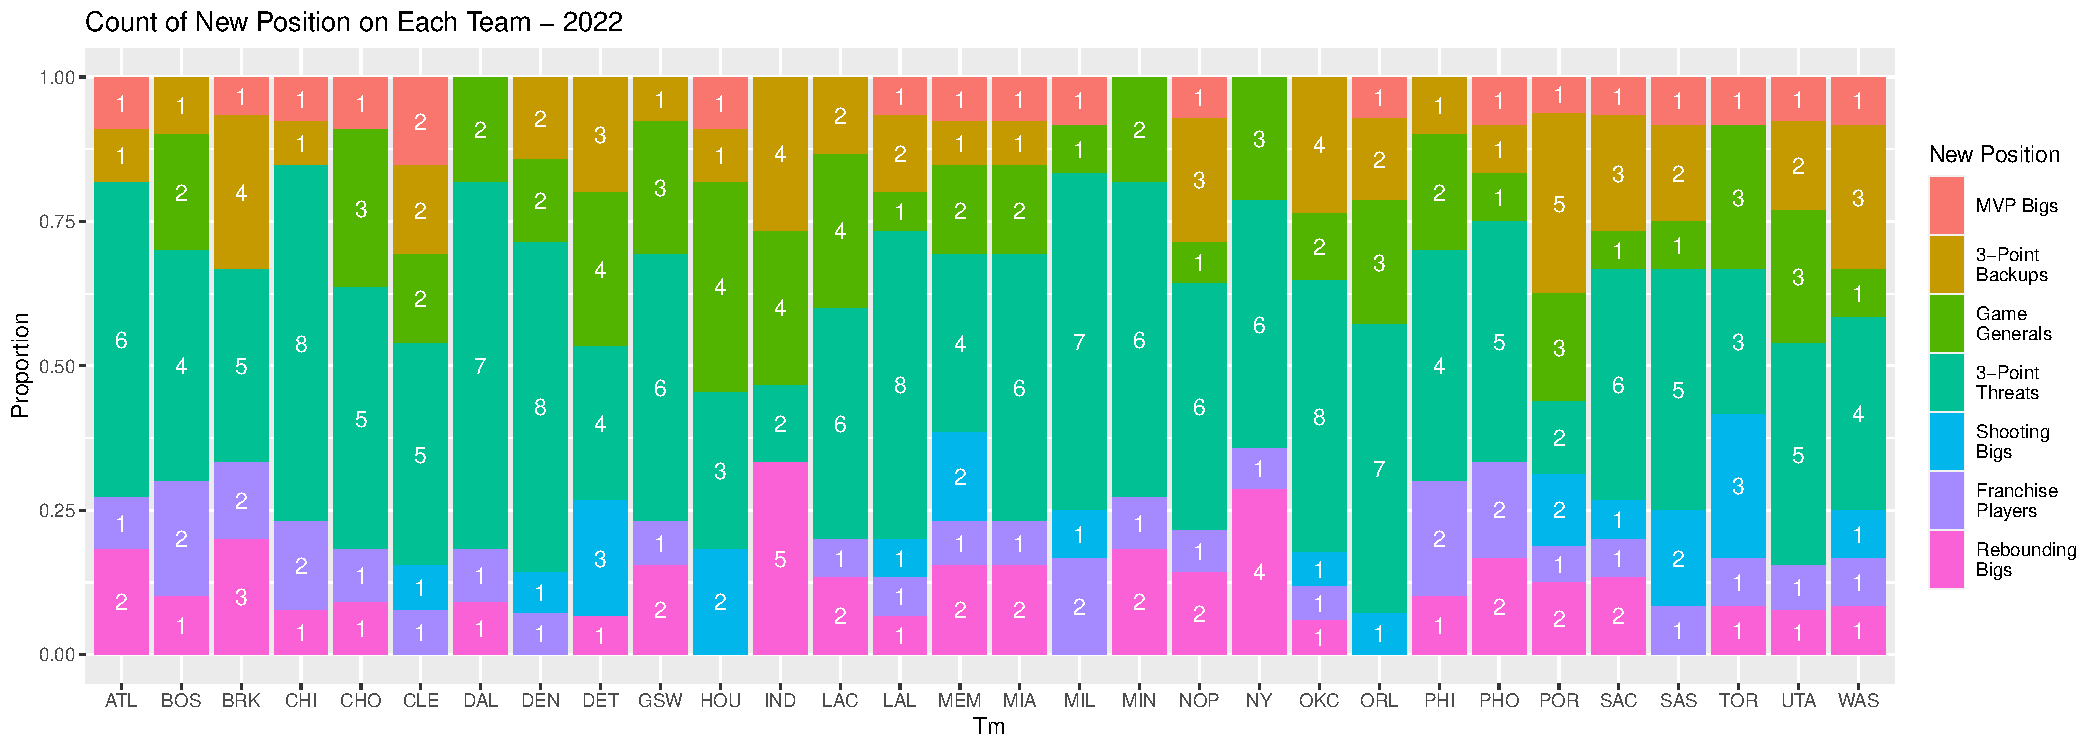
\includegraphics{Reclassifying-NBA-Player-Postions-Pt.-3---Clustering-Analysis-Results_files/figure-latex/unnamed-chunk-14-1.pdf}
\#\# Count of New Position on Each Team Above and below .500- 2022

\begin{Shaded}
\begin{Highlighting}[]
\NormalTok{above500\_2022 }\OtherTok{\textless{}{-}} \FunctionTok{c}\NormalTok{(}\StringTok{\textquotesingle{}PHO\textquotesingle{}}\NormalTok{,}\StringTok{\textquotesingle{}MEM\textquotesingle{}}\NormalTok{,}\StringTok{\textquotesingle{}MIA\textquotesingle{}}\NormalTok{,}\StringTok{\textquotesingle{}GSW\textquotesingle{}}\NormalTok{,}\StringTok{\textquotesingle{}DAL\textquotesingle{}}\NormalTok{,}\StringTok{\textquotesingle{}BOS\textquotesingle{}}\NormalTok{,}\StringTok{\textquotesingle{}MIL\textquotesingle{}}\NormalTok{,}\StringTok{\textquotesingle{}PHI\textquotesingle{}}\NormalTok{,}\StringTok{\textquotesingle{}UTA\textquotesingle{}}\NormalTok{,}\StringTok{\textquotesingle{}TOR\textquotesingle{}}\NormalTok{,}\StringTok{\textquotesingle{}DEN\textquotesingle{}}\NormalTok{,}\StringTok{\textquotesingle{}MIN\textquotesingle{}}\NormalTok{,}\StringTok{\textquotesingle{}CHI\textquotesingle{}}\NormalTok{,}\StringTok{\textquotesingle{}BRK\textquotesingle{}}\NormalTok{,}\StringTok{\textquotesingle{}CLE\textquotesingle{}}\NormalTok{,}\StringTok{\textquotesingle{}ATL\textquotesingle{}}\NormalTok{,}\StringTok{\textquotesingle{}CHO\textquotesingle{}}\NormalTok{,}\StringTok{\textquotesingle{}LAC\textquotesingle{}}\NormalTok{)}

\FunctionTok{ggplot}\NormalTok{(}\AttributeTok{data =}\NormalTok{ df\_2022 }\SpecialCharTok{\%\textgreater{}\%} \FunctionTok{filter}\NormalTok{(Tm }\SpecialCharTok{\%in\%}\NormalTok{ above500\_2022), }\FunctionTok{aes}\NormalTok{(}\AttributeTok{x =}\NormalTok{ Tm, }\AttributeTok{fill =} \FunctionTok{factor}\NormalTok{(Cluster))) }\SpecialCharTok{+}
  \FunctionTok{geom\_bar}\NormalTok{(}\AttributeTok{position =} \StringTok{"fill"}\NormalTok{) }\SpecialCharTok{+} \FunctionTok{ylab}\NormalTok{(}\StringTok{"Proportion by Count"}\NormalTok{) }\SpecialCharTok{+}
  \FunctionTok{stat\_count}\NormalTok{(}\AttributeTok{geom =} \StringTok{"text"}\NormalTok{, }
             \FunctionTok{aes}\NormalTok{(}\AttributeTok{label =} \FunctionTok{stat}\NormalTok{(count)),}
             \AttributeTok{position=}\FunctionTok{position\_fill}\NormalTok{(}\AttributeTok{vjust=}\FloatTok{0.5}\NormalTok{), }\AttributeTok{colour=}\StringTok{"Black"}\NormalTok{) }\SpecialCharTok{+}
      \FunctionTok{scale\_fill\_discrete}\NormalTok{(}\AttributeTok{name =} \StringTok{"New Position"}\NormalTok{, }\AttributeTok{labels =}\FunctionTok{c}\NormalTok{(}\StringTok{\textquotesingle{}MVP Bigs\textquotesingle{}}\NormalTok{, }\StringTok{\textquotesingle{}3{-}Point}\SpecialCharTok{\textbackslash{}n}\StringTok{Backups\textquotesingle{}}\NormalTok{, }\StringTok{\textquotesingle{}Game}\SpecialCharTok{\textbackslash{}n}\StringTok{Generals\textquotesingle{}}\NormalTok{, }\StringTok{\textquotesingle{}3{-}Point}\SpecialCharTok{\textbackslash{}n}\StringTok{Threats\textquotesingle{}}\NormalTok{, }\StringTok{\textquotesingle{}Shooting}\SpecialCharTok{\textbackslash{}n}\StringTok{Bigs\textquotesingle{}}\NormalTok{, }\StringTok{\textquotesingle{}Franchise}\SpecialCharTok{\textbackslash{}n}\StringTok{Players\textquotesingle{}}\NormalTok{, }\StringTok{\textquotesingle{}Rebounding}\SpecialCharTok{\textbackslash{}n}\StringTok{Bigs\textquotesingle{}}\NormalTok{))  }\SpecialCharTok{+}
  \FunctionTok{theme}\NormalTok{(}\AttributeTok{legend.key.height=}\FunctionTok{unit}\NormalTok{(}\DecValTok{1}\NormalTok{, }\StringTok{"cm"}\NormalTok{))}
\end{Highlighting}
\end{Shaded}

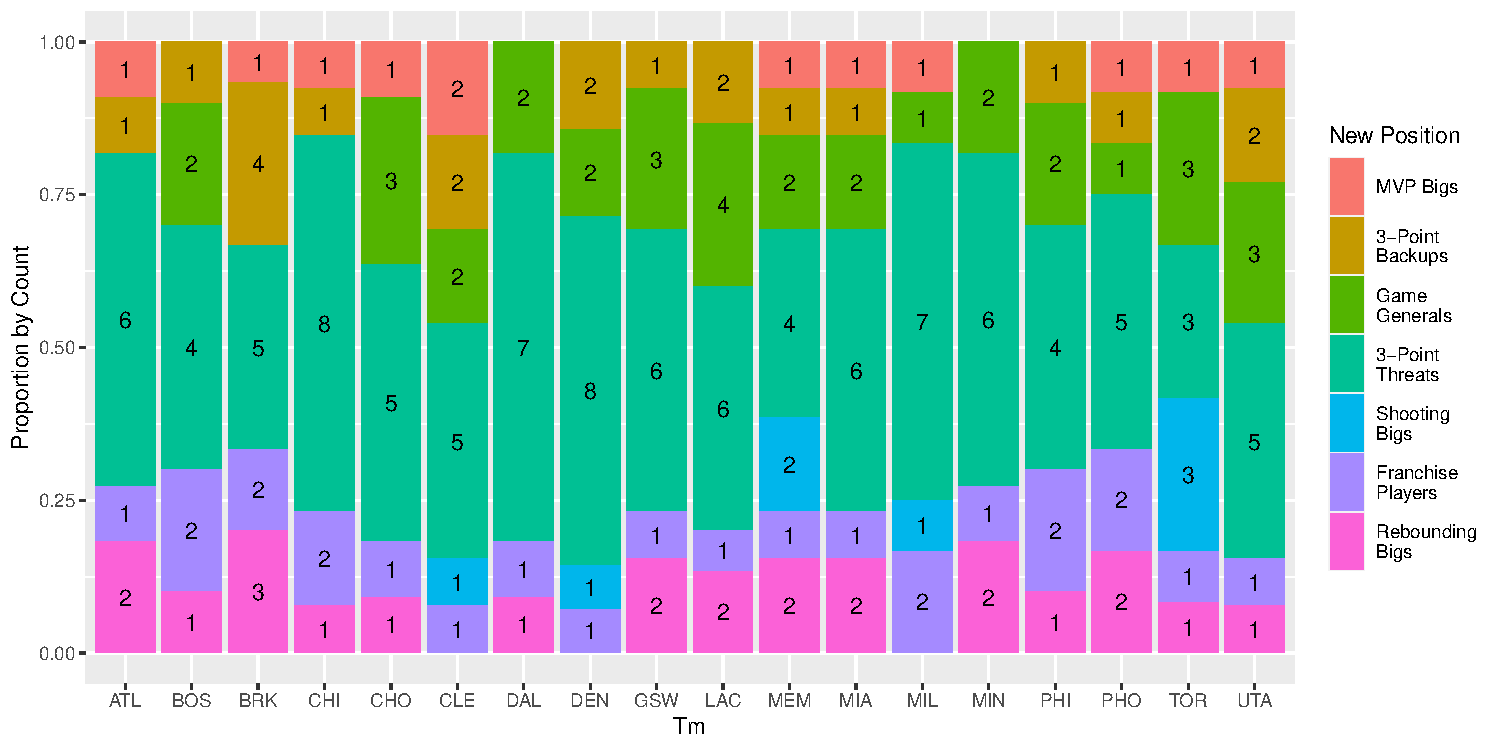
\includegraphics{Reclassifying-NBA-Player-Postions-Pt.-3---Clustering-Analysis-Results_files/figure-latex/unnamed-chunk-15-1.pdf}
\#\#\# Takeaways * Each team with a record above .500 had at least 1
Franchise Player. * Boston, Brooklyn, Chicago, Milwaukee, Philadelphia,
and Phoenix had 2 Franchise Players * Boston, Dallas, Denver, Golden
State, LA Clippers, Minnesota, and Philadelphia didn't have an MVP Big *
Cleveland had 2 MVP Bigs

\hypertarget{count-of-new-position-on-each-team-bwloq-.500--2022}{%
\subsection{Count of New Position on Each Team Bwloq .500-
2022}\label{count-of-new-position-on-each-team-bwloq-.500--2022}}

\begin{Shaded}
\begin{Highlighting}[]
\NormalTok{below500\_2022 }\OtherTok{\textless{}{-}} \FunctionTok{c}\NormalTok{(}\StringTok{\textquotesingle{}NYK\textquotesingle{}}\NormalTok{,}\StringTok{\textquotesingle{}NOP\textquotesingle{}}\NormalTok{,}\StringTok{\textquotesingle{}WAS\textquotesingle{}}\NormalTok{,}\StringTok{\textquotesingle{}SAS\textquotesingle{}}\NormalTok{,}\StringTok{\textquotesingle{}LAL\textquotesingle{}}\NormalTok{,}\StringTok{\textquotesingle{}SAC\textquotesingle{}}\NormalTok{,}\StringTok{\textquotesingle{}POR\textquotesingle{}}\NormalTok{,}\StringTok{\textquotesingle{}IND\textquotesingle{}}\NormalTok{,}\StringTok{\textquotesingle{}OKC\textquotesingle{}}\NormalTok{,}\StringTok{\textquotesingle{}DET\textquotesingle{}}\NormalTok{,}\StringTok{\textquotesingle{}ORL\textquotesingle{}}\NormalTok{,}\StringTok{\textquotesingle{}HOU\textquotesingle{}}\NormalTok{)}
\FunctionTok{ggplot}\NormalTok{(}\AttributeTok{data =}\NormalTok{ df\_2022 }\SpecialCharTok{\%\textgreater{}\%} \FunctionTok{filter}\NormalTok{(Tm }\SpecialCharTok{\%in\%}\NormalTok{ below500\_2022), }\FunctionTok{aes}\NormalTok{(}\AttributeTok{x =}\NormalTok{ Tm, }\AttributeTok{fill =} \FunctionTok{factor}\NormalTok{(Cluster))) }\SpecialCharTok{+}
  \FunctionTok{geom\_bar}\NormalTok{(}\AttributeTok{position =} \StringTok{"fill"}\NormalTok{) }\SpecialCharTok{+} \FunctionTok{ylab}\NormalTok{(}\StringTok{"Proportion by Count"}\NormalTok{) }\SpecialCharTok{+}
  \FunctionTok{stat\_count}\NormalTok{(}\AttributeTok{geom =} \StringTok{"text"}\NormalTok{, }
             \FunctionTok{aes}\NormalTok{(}\AttributeTok{label =} \FunctionTok{stat}\NormalTok{(count)),}
             \AttributeTok{position=}\FunctionTok{position\_fill}\NormalTok{(}\AttributeTok{vjust=}\FloatTok{0.5}\NormalTok{), }\AttributeTok{colour=}\StringTok{"Black"}\NormalTok{) }\SpecialCharTok{+}
      \FunctionTok{scale\_fill\_discrete}\NormalTok{(}\AttributeTok{name =} \StringTok{"New Position"}\NormalTok{, }\AttributeTok{labels =}\FunctionTok{c}\NormalTok{(}\StringTok{\textquotesingle{}MVP Bigs\textquotesingle{}}\NormalTok{, }\StringTok{\textquotesingle{}3{-}Point}\SpecialCharTok{\textbackslash{}n}\StringTok{Backups\textquotesingle{}}\NormalTok{, }\StringTok{\textquotesingle{}Game}\SpecialCharTok{\textbackslash{}n}\StringTok{Generals\textquotesingle{}}\NormalTok{, }\StringTok{\textquotesingle{}3{-}Point}\SpecialCharTok{\textbackslash{}n}\StringTok{Threats\textquotesingle{}}\NormalTok{, }\StringTok{\textquotesingle{}Shooting}\SpecialCharTok{\textbackslash{}n}\StringTok{Bigs\textquotesingle{}}\NormalTok{, }\StringTok{\textquotesingle{}Franchise}\SpecialCharTok{\textbackslash{}n}\StringTok{Players\textquotesingle{}}\NormalTok{, }\StringTok{\textquotesingle{}Rebounding}\SpecialCharTok{\textbackslash{}n}\StringTok{Bigs\textquotesingle{}}\NormalTok{))  }\SpecialCharTok{+}
  \FunctionTok{theme}\NormalTok{(}\AttributeTok{legend.key.height=}\FunctionTok{unit}\NormalTok{(}\DecValTok{1}\NormalTok{, }\StringTok{"cm"}\NormalTok{))}
\end{Highlighting}
\end{Shaded}

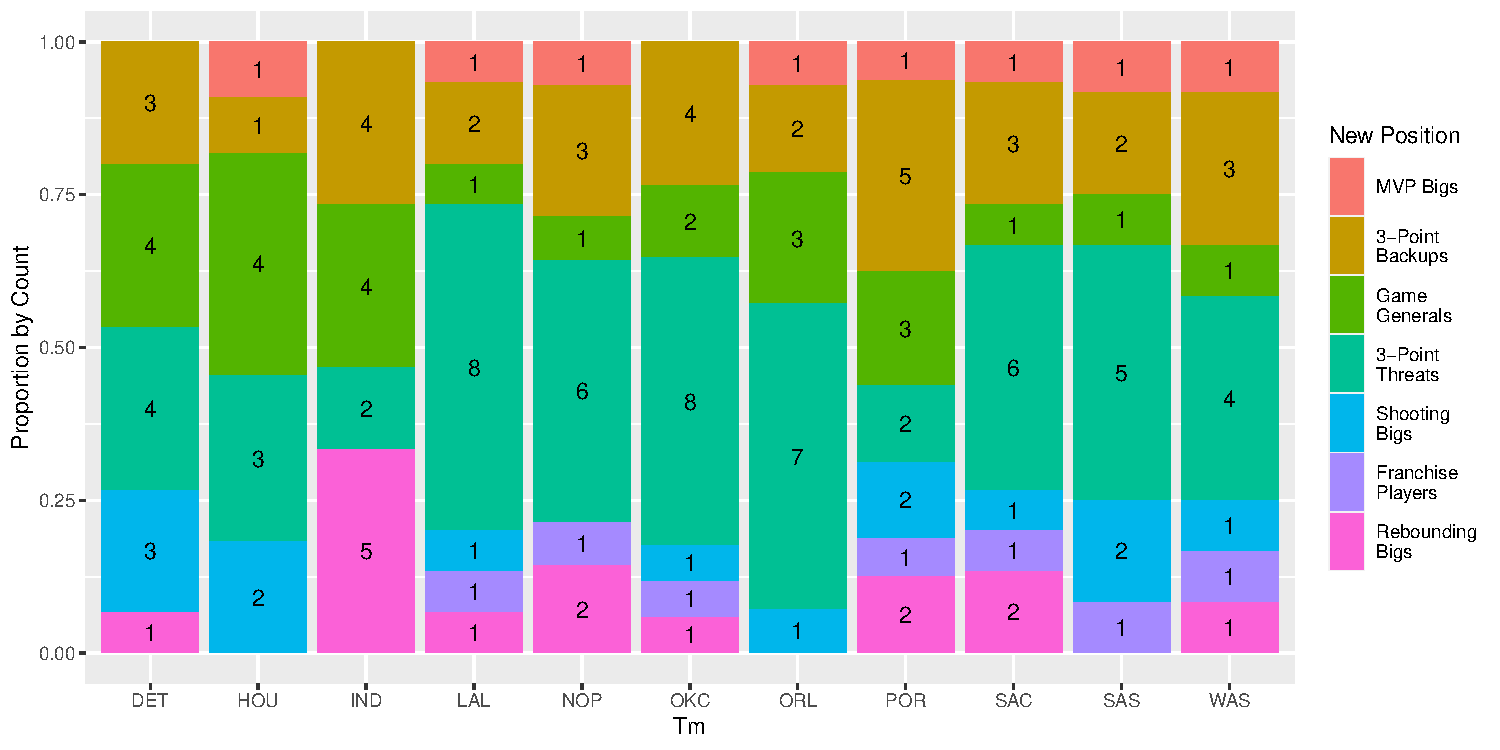
\includegraphics{Reclassifying-NBA-Player-Postions-Pt.-3---Clustering-Analysis-Results_files/figure-latex/unnamed-chunk-16-1.pdf}
\#\#\# Takeaways * 5 of the 11 Teams with a record below .500 didn't
have a Franchise Player. * Of the 5, Detroit and Indiana didn't have an
MVP Big.

\hypertarget{conclusion-and-next-steps}{%
\section{Conclusion and Next Steps}\label{conclusion-and-next-steps}}

Further analysis needs to be done to determine which player types are
included on successful teams. This analysis will be used to help
determine what kind of players to target so that a team can be
successful.

\end{document}
